\mfpicnumber{1}

\opengraphsfile{MoreTrigonometricIdentities}

\setcounter{footnote}{0}

\label{MoreTrigonometricIdentities}

\smallskip

In Section \ref{FundamentalTrigonometricIdentities}, we saw the utility of identities in finding the values of the circular functions of a given angle as well as simplifying expressions involving the circular functions.  In this section, we introduce several collections of identities which have uses in this course and beyond. 

\smallskip

Our first set of identities is the `Even / Odd' identities.  We \textit{observed} the even and odd  properties of the circular functions graphically in Sections \ref{GraphsofSineandCosine} and \ref{GraphsofOtherCircularFunctions}.  Here, we take the time to \textit{prove} these properties from first principles.  We state the theorem below for reference.

\smallskip

\colorbox{ResultColor}{\bbm

\begin{thm} \label{evenodd}  \textbf{Even / Odd Identities:}  For all applicable angles $\theta$, \index{Even/Odd Identities} 

\vspace{-.05in}

\begin{multicols}{3}

\begin{itemize}

\item  $\cos(-\theta) = \cos(\theta)$

\item  $\sec(-\theta) = \sec(\theta)$

\item  $\sin(-\theta) = -\sin(\theta)$

\item  $\csc(-\theta) = -\csc(\theta)$

\item  $\tan(-\theta) = -\tan(\theta)$

\item  $\cot(-\theta) = -\cot(\theta)$

\end{itemize}

\end{multicols}

\end{thm}

\hspace{.1in} 

\vspace*{-.25in}

\ebm}

\smallskip

We start by proving $\cos(-\theta) = \cos(\theta)$ and $\sin(-\theta) = -\sin(\theta)$.  

\smallskip

Consider an angle $\theta$ plotted in standard position. Let $\theta_{\mbox{\tiny $0$}}$ be the angle coterminal with $\theta$ with $0 \leq \theta_{\mbox{\tiny $0$}} < 2\pi$.  (We can construct the angle $\theta_{\mbox{\tiny $0$}}$ by rotating counter-clockwise from the positive $x$-axis to the terminal side of $\theta$ as pictured below.)  Since $\theta$ and $\theta_{\mbox{\tiny $0$}}$ are coterminal, $\cos(\theta) = \cos(\theta_{\mbox{\tiny $0$}})$ and $\sin(\theta) = \sin(\theta_{\mbox{\tiny $0$}})$.

\begin{center}

\begin{tabular}{cc}

\begin{mfpic}[18]{-5}{5}{-4.5}{4.5}
\axes
\tlabel(4.75,-0.5){\scriptsize $x$}
\tlabel(0.25,4.25){\scriptsize $y$}
\tlabel(3.1,-0.75){\scriptsize $1$}
\tlabel(0.25,3.1){\scriptsize $1$}
\xmarks{-3 step 3 until 3}
\ymarks{-3 step 3 until 3}
\drawcolor[gray]{0.7}
\circle{(0,0),3}
\drawcolor{black}
\arrow \parafcn{0,-555,-5}{(-t+400)*dir(t)/800} 
\tlabel(1.5,-1){$\theta$}
\tlabel[cc](-2.5, 2.75){\mbox{\boldmath $\theta_{\mbox{\tiny $0$}}$}}
\point[4pt]{(0,0),(-2.7692, 1.1538)}
\penwd{1.25pt}
\arrow  \reverse \arrow \polyline{(5,0), (0,0), (-4.6154, 1.9231)}
\penwd{1.5pt}
\arrow \parafcn{5, 150, 5}{1.75*dir(t)}
\end{mfpic} 

& 

\begin{mfpic}[18]{-5}{5}{-4.5}{4.5}
\axes
\tlabel(4.75,-0.5){\scriptsize $x$}
\tlabel(0.25,4.25){\scriptsize $y$}
\tlabel(3.1,-0.75){\scriptsize $1$}
\tlabel(0.25,3.1){\scriptsize $1$}
\xmarks{-3 step 3 until 3}
\ymarks{-3 step 3 until 3}
\drawcolor[gray]{0.7}
\circle{(0,0),3}
\drawcolor{black}
\tlabel[cc](-2.5, 2.75){\mbox{\boldmath $\theta_{\mbox{\tiny $0$}}$}}
\tlabel[cc](-2.5, -2.75){\mbox{\boldmath $-\theta_{\mbox{\tiny $0$}}$}}
\point[4pt]{(0,0),(-2.7692, 1.1538)}
\point[4pt]{(0,0),(-2.7692, -1.1538)}
\tlabel(-7,0.75){\scriptsize $P(\cos(\theta_{\mbox{\tiny $0$}}),\sin(\theta_{\mbox{\tiny $0$}}))$}
\tlabel(-7.5,-0.85){\scriptsize $Q(\cos(-\theta_{\mbox{\tiny $0$}}),\sin(-\theta_{\mbox{\tiny $0$}}))$}
\penwd{1.25pt}
\arrow \reverse \arrow \polyline{(5,0), (0,0), (-4.6154, 1.9231)}
\arrow \reverse \arrow \polyline{(5,0), (0,0), (-4.6154, -1.9231)}
\penwd{1.5pt}
\arrow \parafcn{5, 150, 5}{1.75*dir(t)}
\arrow \parafcn{-5, -145, -5}{1.75*dir(t)}
\end{mfpic}  \\

\end{tabular}

\end{center}

We now consider the angles $-\theta$ and $-\theta_{\mbox{\tiny $0$}}$.  Since  $\theta$ is coterminal with $\theta_{\mbox{\tiny $0$}}$, there is some integer $k$ so that $\theta = \theta_{\mbox{\tiny $0$}} + 2\pi \cdot k$.  Hence, $-\theta =   -\theta_{\mbox{\tiny $0$}} - 2\pi \cdot k = -\theta_{\mbox{\tiny $0$}} + 2\pi \cdot(-k)$.  Since $k$ is an integer, so is $(-k)$, which means $-\theta$ is coterminal with $-\theta_{\mbox{\tiny $0$}}$.  Therefore,   $\cos(-\theta) = \cos(-\theta_{\mbox{\tiny $0$}})$ and $\sin(-\theta) = \sin(-\theta_{\mbox{\tiny $0$}})$.  

\smallskip

Let $P$ and $Q$ denote the points on the terminal sides of $\theta_{\mbox{\tiny $0$}}$ and $-\theta_{\mbox{\tiny $0$}}$, respectively, which lie on the Unit Circle. By definition, the coordinates of $P$ are $(\cos(\theta_{\mbox{\tiny $0$}}),\sin(\theta_{\mbox{\tiny $0$}}))$ and the coordinates of $Q$ are $(\cos(-\theta_{\mbox{\tiny $0$}}),\sin(-\theta_{\mbox{\tiny $0$}}))$.  

\smallskip

Since $\theta_{\mbox{\tiny $0$}}$ and $-\theta_{\mbox{\tiny $0$}}$ sweep out congruent central sectors of the Unit Circle, it follows that the points $P$ and $Q$ are symmetric about the $x$-axis.  Thus, $\cos(-\theta_{\mbox{\tiny $0$}}) = \cos(\theta_{\mbox{\tiny $0$}})$ and $\sin(-\theta_{\mbox{\tiny $0$}}) = -\sin(\theta_{\mbox{\tiny $0$}})$. 

\smallskip

Since the cosines and sines of $\theta_{\mbox{\tiny $0$}}$ and $-\theta_{\mbox{\tiny $0$}}$ are the same as those for $\theta$ and $-\theta$, respectively, we get $\cos(-\theta) = \cos(\theta)$ and $\sin(-\theta) = -\sin(\theta)$, as required. 

\smallskip

As we saw in Section \ref{GraphsofOtherCircularFunctions}, the remaining four circular functions `inherit' their even/odd nature from sine and cosine courtesy of the Reciprocal and Quotient Identities, Theorem \ref{recipquotidfull}.  

\smallskip

Our next set of identities establish how the cosine function handles sums and differences of angles.

\smallskip

\colorbox{ResultColor}{\bbm

\begin{thm} \label{cosinesumdifference}  \textbf{Sum and Difference Identities for Cosine:} For all angles $\alpha$ and $\beta$, \index{Difference Identity ! for cosine} \index{Sum Identity ! for cosine}

\begin{itemize}

\item  $\cos(\alpha + \beta) = \cos(\alpha) \cos(\beta) - \sin(\alpha) \sin(\beta)$

\item $\cos(\alpha - \beta) = \cos(\alpha) \cos(\beta) + \sin(\alpha) \sin(\beta)$

\end{itemize}

\end{thm}

\smallskip

\ebm}

\smallskip

We first prove the result for differences.  As in the proof of the Even / Odd Identities, we can reduce the proof for general angles $\alpha$ and $\beta$ to angles $\alpha_{\mbox{\tiny $0$}}$ and $\beta_{\mbox{\tiny $0$}}$, coterminal with $\alpha$ and $\beta$, respectively, each of which measure between $0$ and $2\pi$ radians.  Since $\alpha$ and $\alpha_{\mbox{\tiny $0$}}$ are coterminal, as are $\beta$ and $\beta_{\mbox{\tiny $0$}}$, it follows that $(\alpha - \beta)$ is coterminal with $(\alpha_{\mbox{\tiny $0$}} - \beta_{\mbox{\tiny $0$}})$.  Consider the case below where $\alpha_{\mbox{\tiny $0$}} \geq \beta_{\mbox{\tiny $0$}}$.  

\smallskip

\begin{tabular}{cc}

\begin{mfpic}[25]{-4}{4}{-1}{5}
\axes
\drawcolor[gray]{0.7}
\parafcn{0,180,5}{3*dir(t)}
\drawcolor{black}
\arrow \parafcn{5, 40, 5}{0.75*dir(t)}
\arrow \parafcn{5, 115, 5}{1.35*dir(t)}
\tlabel[cc](0.25,.95){\scriptsize $\alpha_{\mbox{\tiny $0$}}$}
\tlabel[cc](0.95,0.3){\scriptsize $\beta_{\mbox{\tiny $0$}}$}
\tlabel(3.75,-0.5){\scriptsize $x$}
\tlabel(0.25,4.75){\scriptsize $y$}
\tlabel(3,-0.5){\scriptsize $1$}
\tlabel(-0.5,-0.5){\scriptsize $O$}
\xmarks{-3 step 3 until 3}
\ymarks{0 step 3 until 3}
\dotted \polyline{(2.121, 2.121), (-1.5, 2.598)}
\point[4pt]{(0,0), (3,0), (2.121, 2.121), (-1.5, 2.598) }
\tlabel(-4.5,2.5){\scriptsize $P(\cos(\alpha_{\mbox{\tiny $0$}}),\sin(\alpha_{\mbox{\tiny $0$}}))$}
\tlabel(2.5,2){\scriptsize $Q(\cos(\beta_{\mbox{\tiny $0$}}),\sin(\beta_{\mbox{\tiny $0$}}))$}
\penwd{1.5pt}
\arrow \parafcn{50, 115,5}{1.75*dir(t)}
\tlabel(0.1,1.9){\mbox{\scriptsize \boldmath $\alpha_{\mbox{\tiny $0$}} - \beta_{\mbox{\tiny $0$}}$}}
\penwd{1.25pt}
\arrow \reverse \arrow \polyline{(4,0), (0,0), (3.535,3.535)}
\arrow \reverse \arrow \polyline{(4,0), (0,0), (-2.5,4.330)}

\end{mfpic} 

&

\hspace{-0.5in}

\begin{mfpic}[25]{-4}{4}{-1}{5}
\axes
\drawcolor[gray]{0.7}
\parafcn{0,180,5}{3*dir(t)}
\drawcolor{black}
\tlabel(3.75,-0.5){\scriptsize $x$}
\tlabel(0.25,4.75){\scriptsize $y$}
\tlabel(0.25,3.1){\scriptsize $1$}
\tlabel(-0.5,-0.5){\scriptsize $O$}
\xmarks{-3 step 3 until 3}
\ymarks{0 step 3 until 3}

\tlabel(1.25,2.8){\scriptsize $A(\cos(\alpha_{\mbox{\tiny $0$}} - \beta_{\mbox{\tiny $0$}}),\sin(\alpha_{\mbox{\tiny $0$}} - \beta_{\mbox{\tiny $0$}}))$}
\tlabel(2.25,-0.5){\scriptsize $B(1,0)$}
\dotted \polyline{(3,0), (1.026, 2.819)}
\point[4pt]{(0,0), (3,0), (1.026, 2.819)}
\penwd{1.5pt}
\arrow \parafcn{5, 65,5}{1.75*dir(t)}
\tlabel(0.2,0.3){\mbox{\scriptsize \boldmath $\alpha_{\mbox{\tiny $0$}} - \beta_{\mbox{\tiny $0$}}$}}
\penwd{1.25pt}
\arrow \reverse \arrow \polyline{(4,0), (0,0), (1.710,4.698)}
\end{mfpic} 
\end{tabular}

Since the angles $POQ$ and $AOB$ are congruent, the distance between $P$ and $Q$ is equal to the distance between $A$ and $B$.\footnote{In the picture we've drawn, the \underline{tri}angles $POQ$ and $AOB$ are congruent, which is even better.  However, $\alpha_{\mbox{\tiny $0$}} - \beta_{\mbox{\tiny $0$}}$ could be $0$ or it could be $\pi$, neither of which makes a triangle.  It could also be larger than $\pi$, which makes a triangle, just not the one we've drawn.  You should think about those three cases.}  The distance formula, Equation \ref{distanceformula}, yields

\[ \begin{array}{rcl}

\sqrt{(\cos(\alpha_{\mbox{\tiny $0$}}) - \cos(\beta_{\mbox{\tiny $0$}}))^2 + (\sin(\alpha_{\mbox{\tiny $0$}}) - \sin(\beta_{\mbox{\tiny $0$}}))^2 } & = & \sqrt{(\cos(\alpha_{\mbox{\tiny $0$}} - \beta_{\mbox{\tiny $0$}}) - 1)^2 + (\sin(\alpha_{\mbox{\tiny $0$}} - \beta_{\mbox{\tiny $0$}}) - 0)^2} \\ \end{array} \]

Squaring both sides, we expand the left hand side of this equation as

\[ \begin{array}{rcl}
(\cos(\alpha_{\mbox{\tiny $0$}}) - \cos(\beta_{\mbox{\tiny $0$}}))^2 + (\sin(\alpha_{\mbox{\tiny $0$}}) - \sin(\beta_{\mbox{\tiny $0$}}))^2 
& = &  
\cos^2(\alpha_{\mbox{\tiny $0$}}) - 2\cos(\alpha_{\mbox{\tiny $0$}})\cos(\beta_{\mbox{\tiny $0$}}) + \cos^2(\beta_{\mbox{\tiny $0$}}) \\  
& & + \sin^2(\alpha_{\mbox{\tiny $0$}}) - 2\sin(\alpha_{\mbox{\tiny $0$}})\sin(\beta_{\mbox{\tiny $0$}})  +  \sin^2(\beta_{\mbox{\tiny $0$}}) \\ [6pt]
& = & \cos^2(\alpha_{\mbox{\tiny $0$}}) + \sin^2(\alpha_{\mbox{\tiny $0$}}) + \cos^2(\beta_{\mbox{\tiny $0$}}) + \sin^2(\beta_{\mbox{\tiny $0$}}) \\
& & -  2\cos(\alpha_{\mbox{\tiny $0$}})\cos(\beta_{\mbox{\tiny $0$}}) - 2\sin(\alpha_{\mbox{\tiny $0$}})\sin(\beta_{\mbox{\tiny $0$}}) \end{array}\]

From the Pythagorean Identities, $\cos^2(\alpha_{\mbox{\tiny $0$}}) + \sin^2(\alpha_{\mbox{\tiny $0$}}) = 1$ and $\cos^2(\beta_{\mbox{\tiny $0$}}) + \sin^2(\beta_{\mbox{\tiny $0$}}) = 1$, so

\[ \begin{array}{rcl}
(\cos(\alpha_{\mbox{\tiny $0$}}) - \cos(\beta_{\mbox{\tiny $0$}}))^2 + (\sin(\alpha_{\mbox{\tiny $0$}}) - \sin(\beta_{\mbox{\tiny $0$}}))^2 
& = & 2  - 2\cos(\alpha_{\mbox{\tiny $0$}})\cos(\beta_{\mbox{\tiny $0$}}) - 2\sin(\alpha_{\mbox{\tiny $0$}})\sin(\beta_{\mbox{\tiny $0$}}) \end{array}\]

Turning our attention to the right hand side of our equation, we find

\[ \begin{array}{rcl}
(\cos(\alpha_{\mbox{\tiny $0$}} - \beta_{\mbox{\tiny $0$}}) - 1)^2 + (\sin(\alpha_{\mbox{\tiny $0$}} - \beta_{\mbox{\tiny $0$}}) - 0)^2 & = & \cos^2(\alpha_{\mbox{\tiny $0$}} - \beta_{\mbox{\tiny $0$}}) - 2\cos(\alpha_{\mbox{\tiny $0$}} - \beta_{\mbox{\tiny $0$}}) + 1 + \sin^2(\alpha_{\mbox{\tiny $0$}} - \beta_{\mbox{\tiny $0$}}) \\ 
& = & 1 +  \cos^2(\alpha_{\mbox{\tiny $0$}} - \beta_{\mbox{\tiny $0$}}) + \sin^2(\alpha_{\mbox{\tiny $0$}} - \beta_{\mbox{\tiny $0$}}) - 2\cos(\alpha_{\mbox{\tiny $0$}} - \beta_{\mbox{\tiny $0$}}) \\
\end{array} \]

Once again, we simplify $\cos^2(\alpha_{\mbox{\tiny $0$}} - \beta_{\mbox{\tiny $0$}}) + \sin^2(\alpha_{\mbox{\tiny $0$}} - \beta_{\mbox{\tiny $0$}})= 1$, so that

\[ \begin{array}{rcl}
(\cos(\alpha_{\mbox{\tiny $0$}} - \beta_{\mbox{\tiny $0$}}) - 1)^2 + (\sin(\alpha_{\mbox{\tiny $0$}} - \beta_{\mbox{\tiny $0$}}) - 0)^2 & = & 2  - 2\cos(\alpha_{\mbox{\tiny $0$}} - \beta_{\mbox{\tiny $0$}}) \\ \end{array} \]

Putting it all together, we get $2  - 2\cos(\alpha_{\mbox{\tiny $0$}})\cos(\beta_{\mbox{\tiny $0$}}) - 2\sin(\alpha_{\mbox{\tiny $0$}})\sin(\beta_{\mbox{\tiny $0$}}) = 2  - 2\cos(\alpha_{\mbox{\tiny $0$}} - \beta_{\mbox{\tiny $0$}})$, which simplifies to: $\cos(\alpha_{\mbox{\tiny $0$}} - \beta_{\mbox{\tiny $0$}}) = \cos(\alpha_{\mbox{\tiny $0$}})\cos(\beta_{\mbox{\tiny $0$}}) + \sin(\alpha_{\mbox{\tiny $0$}})\sin(\beta_{\mbox{\tiny $0$}})$. 

\smallskip

Since $\alpha$ and $\alpha_{\mbox{\tiny $0$}}$, $\beta$ and $\beta_{\mbox{\tiny $0$}}$, and $(\alpha - \beta)$ and $(\alpha_{\mbox{\tiny $0$}}- \beta_{\mbox{\tiny $0$}})$ are all coterminal pairs of angles, we have established the identity: $\cos(\alpha - \beta) = \cos(\alpha) \cos(\beta) + \sin(\alpha) \sin(\beta)$. 

\smallskip

For the case where $\alpha_{\mbox{\tiny $0$}} \leq \beta_{\mbox{\tiny $0$}}$, we can apply the above argument to the angle $\beta_{\mbox{\tiny $0$}} - \alpha_{\mbox{\tiny $0$}}$ to obtain the identity  $\cos(\beta_{\mbox{\tiny $0$}} - \alpha_{\mbox{\tiny $0$}}) = \cos(\beta_{\mbox{\tiny $0$}})\cos(\alpha_{\mbox{\tiny $0$}}) + \sin(\beta_{\mbox{\tiny $0$}})\sin(\alpha_{\mbox{\tiny $0$}})$.  Using this formula in conjunction with  the  Even Identity of cosine gives us the result in this case, too: 

\[ \begin{array}{rcl}  \cos(\alpha_{\mbox{\tiny $0$}} - \beta_{\mbox{\tiny $0$}}) =  \cos( - (\alpha_{\mbox{\tiny $0$}} - \beta_{\mbox{\tiny $0$}}))  =  \cos(\beta_{\mbox{\tiny $0$}} - \alpha_{\mbox{\tiny $0$}})  & = & \cos(\beta_{\mbox{\tiny $0$}})\cos(\alpha_{\mbox{\tiny $0$}}) + \sin(\beta_{\mbox{\tiny $0$}})\sin(\alpha_{\mbox{\tiny $0$}}) \\
& = & \cos(\alpha_{\mbox{\tiny $0$}})\cos(\beta_{\mbox{\tiny $0$}}) + \sin(\alpha_{\mbox{\tiny $0$}})\sin(\beta_{\mbox{\tiny $0$}}). \end{array} \]

\medskip

To get the sum identity for cosine, we use the difference formula along with the Even/Odd Identities

\vspace{-.15in}

\[ \cos(\alpha + \beta) = \cos(\alpha - (-\beta)) =  \cos(\alpha) \cos(-\beta) + \sin(\alpha) \sin(-\beta) =  \cos(\alpha) \cos(\beta) - \sin(\alpha) \sin(\beta).  \]

We put these newfound identities to good use in the following example.

\begin{ex} \label{cosinesumdiffex}  $~$

\begin{enumerate}

\item Find the exact value of $\cos\left(15^{\circ}\right)$.

\item  Verify the identity:  $\cos\left(\frac{\pi}{2} - \theta\right) = \sin(\theta)$.

\item  Suppose $\alpha$ is a Quadrant I angle with $\sin(\alpha) = \frac{3}{5}$ and $\beta$ is a Quadrant IV angle with $\sec(\beta) = 4$.  Find the exact value of $\cos(\alpha + \beta)$.


\end{enumerate}

{\bf Solution.}

\begin{enumerate}

\item In order to use Theorem \ref{cosinesumdifference} to find $\cos\left(15^{\circ}\right)$, we need to write $15^{\circ}$ as a sum or difference of angles whose cosines and sines we know.  One way to do so is to write $15^{\circ} = 45^{\circ} - 30^{\circ}$.  We find:

\[ \begin{array}{rcl}

\cos\left(15^{\circ}\right) & = & \cos\left(45^{\circ} - 30^{\circ} \right) \\ [2pt]
                            & = & \cos\left(45^{\circ}\right)\cos\left(30^{\circ} \right) + \sin\left(45^{\circ}\right)\sin\left(30^{\circ} \right) \\ [2pt]
                            & = & \left( \dfrac{\sqrt{2}}{2} \right)\left( \dfrac{\sqrt{3}}{2} \right)  +  \left( \dfrac{\sqrt{2}}{2} \right)\left( \dfrac{1}{2} \right)\\ [15pt]
														& = &  \dfrac{\sqrt{6}+ \sqrt{2}}{4}. \\ 
\end{array} \]


\item Using Theorem \ref{cosinesumdifference} gives:

\[ \begin{array}{rcl}

\cos\left(\dfrac{\pi}{2} - \theta\right) & = & \cos\left(\dfrac{\pi}{2}\right)\cos\left(\theta\right) + \sin\left(\dfrac{\pi}{2}\right)\sin\left(\theta \right) \\ [10pt]
                            & = & \left( 0 \right)\left( \cos(\theta) \right)  +  \left( 1 \right)\left( \sin(\theta) \right) \\ [4pt]
														& = & \sin(\theta) .   \\
\end{array} \]

\item  Per Theorem \ref{cosinesumdifference}, we know $\cos(\alpha + \beta) = \cos(\alpha) \cos(\beta) - \sin(\alpha) \sin(\beta)$.  Hence, we need to find the sines and cosines of $\alpha$ and $\beta$ to complete the problem.

\smallskip

We are given  $\sin(\alpha) = \frac{3}{5}$, so our first task is to find $\cos(\alpha)$.  We can quickly get $\cos(\alpha)$ using the Pythagorean Identity $\cos^{2}(\alpha) = 1 - \sin^{2}(\alpha) = 1 - \left(\frac{3}{5}\right)^2 = \frac{16}{25}$.  We get $\cos(\alpha) =  \frac{4}{5}$, choosing the positive root  since $\alpha$ is a Quadrant I angle.

\smallskip

Next, we need the $\sin(\beta)$ and $\cos(\beta)$.  Since $\sec(\beta) = 4$, we immediately get $\cos(\beta) = \frac{1}{4}$ courtesy of the Reciprocal and Quotient Identities.  

\smallskip

To get $\sin(\beta)$, we employ the Pythagorean Identity: $\sin^{2}(\beta) = 1 - \cos^{2}(\beta) = 1 - \left(\frac{1}{4} \right)^2 = \frac{15}{16}$.  Here, since $\beta$ is a Quadrant IV angle, we get $\sin(\beta) =  - \frac{\sqrt{15}}{4}$.

\smallskip

Finally, we get: $\cos(\alpha + \beta) = \cos(\alpha) \cos(\beta) - \sin(\alpha) \sin(\beta) = \left( \frac{4}{5} \right)  \left( \frac{1}{4} \right)  -  \left( \frac{3}{5} \right)   \left( - \frac{\sqrt{15}}{4} \right)  = \frac{4+3\sqrt{15}}{20}$. \qed


\end{enumerate}


\end{ex}

The identity verified in Example \ref{cosinesumdiffex}, namely, $\cos\left(\frac{\pi}{2} - \theta\right) = \sin(\theta)$,  is the first of the celebrated `cofunction' identities.  These identities were first hinted at in Exercise \ref{cofunctionforeshadowing} in Section \ref{AppRightTrig}. 

\smallskip

From $ \sin(\theta) = \cos\left(\frac{\pi}{2} - \theta\right) $, we get:  $\sin\left(\frac{\pi}{2} - \theta\right) = \cos\left(\frac{\pi}{2} -\left[\frac{\pi}{2} - \theta\right]\right) = \cos(\theta)$, which says, in words,  that the `co'sine of an angle is the sine of its `co'mplement.  Now that these identities have been established for cosine and sine, the remaining circular functions follow suit.  The remaining proofs are left as exercises.

\medskip

\colorbox{ResultColor}{\bbm

\begin{thm} \label{cofunctionidentities}  \textbf{Cofunction Identities:} For all applicable angles $\theta$, \index{Cofunction Identities}

\begin{multicols}{3}

\begin{itemize}

\item  $\cos\left(\dfrac{\pi}{2} - \theta \right) = \sin(\theta)$

\item  $\sin\left(\dfrac{\pi}{2} - \theta \right) = \cos(\theta)$

\item  $\sec\left(\dfrac{\pi}{2} - \theta \right) = \csc(\theta)$

\item  $\csc\left(\dfrac{\pi}{2} - \theta \right) = \sec(\theta)$

\item  $\tan\left(\dfrac{\pi}{2} - \theta \right) = \cot(\theta)$

\item  $\cot\left(\dfrac{\pi}{2} - \theta \right) = \tan(\theta)$

\end{itemize}

\end{multicols}

\end{thm}

\vspace{.01in}

\ebm}

\medskip

The Cofunction Identities enable us to derive the sum and difference formulas for sine.  We first convert to sine to cosine and expand:
\[ \begin{array}{rcl}

\sin(\alpha + \beta) & = & \cos\left( \dfrac{\pi}{2} - (\alpha + \beta) \right) \\ [10pt]
                     & = & \cos\left( \left[\dfrac{\pi}{2} - \alpha \right] - \beta \right) \\ [10pt]
                     & = & \cos\left(\dfrac{\pi}{2} - \alpha \right) \cos(\beta) + \sin\left(\dfrac{\pi}{2} - \alpha \right)\sin(\beta) \\ [10pt]
                     & = & \sin(\alpha) \cos(\beta) + \cos(\alpha) \sin(\beta) \\ \end{array} \]


We can derive the difference formula for sine by rewriting  $\sin(\alpha - \beta)$ as $\sin(\alpha + (-\beta))$ and using the sum formula and the Even / Odd Identities. Again, we leave the details to the reader.

\medskip

\colorbox{ResultColor}{\bbm

\begin{thm} \label{sinesumdifference}  \textbf{Sum and Difference Identities for Sine:} For all angles $\alpha$ and $\beta$, \index{Difference Identity ! for sine} \index{Sum Identity ! for sine}

\begin{itemize}

\item  $\sin(\alpha + \beta) = \sin(\alpha) \cos(\beta) + \cos(\alpha) \sin(\beta)$

\item $\sin(\alpha - \beta) = \sin(\alpha) \cos(\beta) - \cos(\alpha) \sin(\beta)$

\end{itemize}

\end{thm}

\smallskip

\ebm}

\smallskip

We try out these new identities in the next example.

\smallskip

\begin{ex} $~$  \label{sinesumanddiffex}

\begin{enumerate}

\item  Find the exact value of $\sin\left(\frac{19 \pi}{12}\right)$

\item  Suppose $\alpha$ is a Quadrant II angle with $\sin(\alpha) = \frac{5}{13}$, and $\beta$ is a Quadrant III angle with $\tan(\beta) = 2$. Find the exact value of $\sin(\alpha - \beta)$.

\item  Derive a formula for $\tan(\alpha + \beta)$ in terms of $\tan(\alpha)$ and $\tan(\beta)$.

\end{enumerate}

{\bf Solution.}  

\begin{enumerate}

\item  As in  Example \ref{cosinesumdiffex}, we need to write the angle $\frac{19 \pi}{12}$ as a sum or difference of common angles.  The denominator of $12$ suggests a combination of angles with denominators $3$ and $4$.  One such combination\footnote{It takes some trial and error  to find this combination.  One alternative is to convert to degrees \ldots} is $\; \frac{19 \pi}{12} = \frac{4 \pi}{3} + \frac{\pi}{4}$.  Applying Theorem \ref{sinesumdifference}, we get

\vspace{-.15in}

\[ \begin{array}{rcl}

\sin\left(\dfrac{19 \pi}{12}\right) & = & \sin\left(\dfrac{4 \pi}{3} + \dfrac{\pi}{4} \right) \\ [10pt]
                            & = & \sin\left(\dfrac{4 \pi}{3} \right)\cos\left(\dfrac{\pi}{4} \right) + \cos\left(\dfrac{4 \pi}{3} \right)\sin\left(\dfrac{\pi}{4} \right) \\ [10pt]
                            & = & \left( -\dfrac{\sqrt{3}}{2} \right)\left( \dfrac{\sqrt{2}}{2} \right)  +  \left( -\dfrac{1}{2} \right)\left( \dfrac{\sqrt{2}}{2} \right) \\ [15pt]
														& = &  \dfrac{-\sqrt{6}- \sqrt{2}}{4} \\
\end{array} \]

\vspace{-.1in}

\item  In order to find $\sin(\alpha - \beta)$ using Theorem \ref{sinesumdifference}, we need to find $\cos(\alpha)$ and both $\cos(\beta)$ and $\sin(\beta)$.  

\smallskip

To find $\cos(\alpha)$, we use the Pythagorean Identity $\cos^2(\alpha) = 1 - \sin^{2}(\alpha) = 1 -  \left(\frac{5}{13}\right)^2 = \frac{144}{169}$.   We get $\cos(\alpha) = -\frac{12}{13}$, the negative, here, owing to the fact that $\alpha$ is a Quadrant II angle.

\smallskip

 We now set about finding $\sin(\beta)$ and $\cos(\beta)$.   We have several ways to proceed at this point, but since there isn't a direct way to get from $\tan(\beta)  = 2$ to either $\sin(\beta)$ or $\cos(\beta)$, we opt for a more geometric approach as presented in Section \ref{TheOtherCircularFunctions}. 
 \smallskip
 
 Since $\beta$ is a Quadrant III angle with $\tan(\beta) = 2 = \frac{-2}{-1}$, we know the point $Q(x,y) = (-1,-2)$ is on the terminal side of $\beta$ as illustrated below.\footnote{Note that even though $\tan(\beta) = \frac{\sin(\beta)}{\cos(\beta)}$,  we \textit{cannot} take $\sin(\beta)=-2$ and $\cos(\beta) = -1$.   Recall that $\sin(\beta)$ and $\cos(\beta)$ are the $y$ and $x$ coordinates on a \textit{specific} circle, the Unit Circle.  As we'll see shortly, $(-1,-2)$ lies on a circle of $\sqrt{5}$, so \textit{not} the Unit Circle.}

 \begin{center}
 
\begin{mfpic}[18]{-5}{5}{-4}{4.75}
\axes
\tlabel(4.75,-0.5){\scriptsize $x$}
\tlabel(0.25,4.5){\scriptsize $y$}
\tlabel[cc](-3,-3){\scriptsize $(-1,-2)$}
\tlabel[cc](-2,-1.5){\scriptsize $r=\sqrt{5}$}
\tcaption{the terminal side of $\beta$ contains $Q(-1,-2)$}
\xmarks{-3, -1.5,  1.5, 3}
\ymarks{-3, -1.5,  1.5, 3}
\drawcolor[gray]{0.7}
\circle{(0,0),3.354}
\drawcolor{black}
\penwd{1.25pt}
\arrow \reverse \arrow \polyline{(5,0),(0,0), (-1.79, -3.58)}
\point[4pt]{(0,0), (-1.5, -3)}
\tlpointsep{4pt}
\scriptsize 
\axislabels {x}{ {$-2 \hspace{7pt}$} -3, {$-1 \hspace{7pt}$} -1.5,  {$1$} 1.5,  {$2$} 3}
\axislabels {y}{ {$-2$} -3, {$-1$} -1.5, {$2$} 3, {$1$} 1.5}
\normalsize
\end{mfpic}
 
 
 \end{center}
 
 We find $r = \sqrt{x^2 + y^2} = \sqrt{(-1)^2+(-2)^2} = \sqrt{5}$, so per Theorem \ref{circularfunctionscircle}, $\sin(\beta) = \frac{-2}{\sqrt{5}} = - \frac{2\sqrt{5}}{5}$ and $\cos(\beta) = \frac{-1}{\sqrt{5}} = - \frac{\sqrt{5}}{5}$ .
 
 \smallskip

At last, we have $\sin(\alpha - \beta) = \sin(\alpha)\cos(\beta) - \cos(\alpha)\sin(\beta) =  \left( \frac{5}{13} \right)\left( -\frac{\sqrt{5}}{5} \right) - \left( -\frac{12}{13} \right)\left( - \frac{2 \sqrt{5}}{5} \right)  = -\frac{29\sqrt{5}}{65}$.

\item  We can start expanding $\tan(\alpha + \beta)$ using a quotient identity and our sum formulas

\vspace{-.1in}

\[ \begin{array}{rcl}

\tan(\alpha + \beta) & = & \dfrac{\sin(\alpha + \beta)}{\cos(\alpha + \beta)} \\ [10pt]
                     & = & \dfrac{\sin(\alpha) \cos(\beta) + \cos(\alpha) \sin(\beta)}{\cos(\alpha) \cos(\beta) - \sin(\alpha) \sin(\beta)} \\ \end{array} \]
			

Since  $\tan(\alpha) = \frac{\sin(\alpha)}{\cos(\alpha)}$ and $\tan(\beta) = \frac{\sin(\beta)}{\cos(\beta)}$, it looks as though if we divide both numerator and denominator by $\cos(\alpha) \cos(\beta)$ we will have what we want

\vspace{-.1in}

\[ \begin{array}{rcl}

\tan(\alpha + \beta) & = & \dfrac{\sin(\alpha) \cos(\beta) + \cos(\alpha) \sin(\beta)}{\cos(\alpha) \cos(\beta) - \sin(\alpha) \sin(\beta)} \cdot\dfrac{\dfrac{1}{\cos(\alpha) \cos(\beta)}}{\dfrac{1}{\cos(\alpha) \cos(\beta)}}\\
                    &   & \\
 										& = & \dfrac{\dfrac{\sin(\alpha) \cos(\beta)}{\cos(\alpha) \cos(\beta)} + \dfrac{\cos(\alpha) \sin(\beta)}{\cos(\alpha) \cos(\beta)}}{\dfrac{\cos(\alpha) \cos(\beta)}{\cos(\alpha) \cos(\beta)} - \dfrac{\sin(\alpha) \sin(\beta)}{\cos(\alpha) \cos(\beta)}}\\
                    &   & \\
										& = & \dfrac{\dfrac{\sin(\alpha) \cancel{\cos(\beta)}}{\cos(\alpha) \cancel{\cos(\beta)}} + \dfrac{\cancel{\cos(\alpha)} \sin(\beta)}{\cancel{\cos(\alpha)} \cos(\beta)}}{\dfrac{\cancel{\cos(\alpha)} \cancel{\cos(\beta)}}{\cancel{\cos(\alpha)} \cancel{\cos(\beta)}} - \dfrac{\sin(\alpha) \sin(\beta)}{\cos(\alpha) \cos(\beta)}}\\
                    &   & \\
										& = & \dfrac{\tan(\alpha) + \tan(\beta)}{1 -\tan(\alpha) \tan(\beta)}\\
\end{array} \]

Naturally, this formula is limited to those cases where all of the tangents are defined.\qed

\end{enumerate}

\end{ex}

The formula developed in Exercise \ref{sinesumanddiffex} for $\tan(\alpha + \beta)$ can be used to find a formula for $\tan(\alpha - \beta)$ by rewriting the difference as a sum, $\tan(\alpha + (-\beta))$ and using the odd property of tangent.  (The reader is encouraged to fill in the details.)  Below we summarize all of the sum and difference formulas.

\smallskip

\colorbox{ResultColor}{\bbm

\begin{thm} \label{circularsumdifference}  \textbf{Sum and Difference Identities:} For all applicable angles $\alpha$ and $\beta$, \index{Difference Identity ! for tangent} \index{Sum Identity ! for tangent} \index{Difference Identity ! for cosine} \index{Sum Identity ! for cosine} \index{Difference Identity ! for sine} \index{Sum Identity ! for sine}

\begin{itemize}

\item  $\cos(\alpha \pm \beta) = \cos(\alpha) \cos(\beta) \mp \sin(\alpha) \sin(\beta)$

\item  $\sin(\alpha \pm \beta) = \sin(\alpha) \cos(\beta) \pm \cos(\alpha) \sin(\beta)$

\item $\tan(\alpha \pm \beta) = \dfrac{\tan(\alpha) \pm \tan(\beta)}{1 \mp \tan(\alpha) \tan(\beta)}$

\end{itemize}

\end{thm}

\smallskip

\ebm}

\smallskip

In the statement of Theorem \ref{circularsumdifference}, we have combined the cases for the sum `$+$' and difference `$-$' of angles into one formula.  The convention here is that if you want the formula for the sum `$+$' of two angles, you use the top sign in the formula;  for the difference, `$-$', use the bottom sign.  For example, \[\tan(\alpha - \beta) = \dfrac{\tan(\alpha) - \tan(\beta)}{1 + \tan(\alpha) \tan(\beta)}\]

If we set $\alpha = \beta$  in the sum formulas in Theorem \ref{circularsumdifference}, we obtain the following `Double Angle' Identities:

\smallskip

\colorbox{ResultColor}{\bbm

\begin{thm} \label{doubleangle}  \textbf{Double Angle Identities:} For all applicable angles $\theta$, \index{Double Angle Identities}

\begin{itemize}

\item  $\cos(2\theta) = \left\{ \begin{array}{l} \cos^{2}(\theta) - \sin^{2}(\theta)\\ [5pt]  2\cos^{2}(\theta) - 1 \\ [5pt] 1-2\sin^{2}(\theta) \end{array} \right.$

\item $\sin(2\theta) = 2\sin(\theta)\cos(\theta)$

\item  $\tan(2\theta) = \dfrac{2\tan(\theta)}{1 - \tan^{2}(\theta)}$

\end{itemize}

\end{thm}

\smallskip

\ebm}

\smallskip

The three different forms for $\cos(2\theta)$ can be explained by our ability to `exchange' squares of cosine and sine via the Pythagorean Identity.  For instance, if we substitute $\sin^{2}(\theta) = 1 - \cos^{2}(\theta)$ into the first  formula for $\cos(2\theta)$, we get $\cos(2\theta)  = \cos^{2}(\theta) - \sin^{2}(\theta) = \cos^{2}(\theta) - (1 - \cos^{2}(\theta)) = 2 \cos^{2}(\theta) - 1$. 

\smallskip

 It is interesting to note that to determine the value of $\cos(2\theta)$, only \textit{one} piece of information is required: either $\cos(\theta)$ or $\sin(\theta)$.  To determine $\sin(2\theta)$, however, it appears that we must know both $\sin(\theta)$ and $\cos(\theta)$.  In the next example, we show how we can find $\sin(2\theta)$ knowing just one piece of information, namely $\tan(\theta)$.

\begin{ex}  \label{doubleangleex} $~$

\begin{enumerate}

\item Suppose $P(-3,4)$ lies on the terminal side of $\theta$ when $\theta$ is plotted in standard position. 

\smallskip

 Find $\cos(2\theta)$ and $\sin(2\theta)$ and determine the quadrant in which the terminal side of the angle $2\theta$ lies when it is plotted in standard position.

\item  If $\sin(\theta) = x$ for $-\frac{\pi}{2} \leq \theta \leq \frac{\pi}{2}$, find an expression for $\sin(2\theta)$ in terms of $x$.

\item  \label{doubleanglesinewtan} Verify the identity:  $\sin(2\theta) = \dfrac{2\tan(\theta)}{1 + \tan^{2}(\theta)}$.

\item  Express $\cos(3\theta)$ as a polynomial in terms of $\cos(\theta)$.
\label{cosinepolynomial}

\end{enumerate}


{\bf Solution.}

\begin{enumerate}

\item  We sketch the terminal side of $\theta$ below on the left.  Using Theorem \ref{cosinesinecircle} from Section \ref{TheCircularFunctionsSineandCosine} with  $x = -3$ and $y=4$, we find $r = \sqrt{x^2+y^2} = 5$.  Hence, $\cos(\theta) = -\frac{3}{5}$ and $\sin(\theta) = \frac{4}{5}$.  

\smallskip

 Theorem \ref{doubleangle} gives us three different formulas to choose from to find $\cos(2\theta)$. Using the first formula,\footnote{We invite the reader to check this answer using the other two formulas.} we get: $\cos(2\theta) = \cos^{2}(\theta) - \sin^{2}(\theta) = \left(-\frac{3}{5}\right)^2 - \left(\frac{4}{5}\right)^2 = -\frac{7}{25}$.    For $\sin(2\theta)$, we get $\sin(2\theta) = 2 \sin(\theta) \cos(\theta) = 2 \left(\frac{4}{5}\right)\left(-\frac{3}{5}\right) = -\frac{24}{25}$.  

\smallskip

Since both cosine and sine of $2\theta$ are negative, the terminal side of $2\theta$, when plotted in standard position, lies in Quadrant III.  To see this more clearly, we plot the terminal side of $2\theta$, along with the terminal side of $\theta$ below on the right.  

\smallskip

Note that in order to find the point $Q(x,y)$ on the terminal side of $2\theta$ of a circle of radius $5$, we use Theorem \ref{cosinesinecircle}  again and find $x = r \cos(2\theta) = 5 \left(-\frac{7}{25} \right) = -\frac{7}{5}$ and $y = r \sin(2\theta) =  5 \left(-\frac{24}{25}\right) = -\frac{24}{5}$.

\smallskip


\begin{center}

\begin{multicols}{2}

\begin{mfpic}[18]{-5}{5}{-5}{5}
\axes
\tlabel(4.75,-0.5){\scriptsize $x$}
\tlabel(0.25,4.5){\scriptsize $y$}
\tlabel(-4.25,2.75){\scriptsize $P(-3,4)$}
\tlabel[cc](-2,1.5){\scriptsize $r=5$}
\tcaption{$P(-3,4)$ is on the terminal side of $\theta$. \vphantom{$Q\left( -\frac{7}{5}, -\frac{24}{5}\right)$}}
\xmarks{-2.68, -2,  -1.34, -0.67, 0.67, 1.34, 2, 2.68}
\ymarks{-2.68, -2,  -1.34, -0.67, 0.67, 1.34, 2, 2.68}
\drawcolor[gray]{0.7}
\circle{(0,0),3.354}
\drawcolor{black}
\penwd{1.25pt}
\arrow \reverse \arrow \polyline{(5,0),(0,0), (-3, 4)}
\point[4pt]{(0,0), (-2.012, 2.683)}
\tlpointsep{4pt}
\scriptsize 
\axislabels {x}{ {$-3 \hspace{7pt}$} -2, {$-1 \hspace{7pt}$} -0.67,  {$1$} 0.67,  {$3$} 2, {$-2 \hspace{7pt}$} -1.34, {$-4 \hspace{7pt}$} -2.68, {$2$} 1.34, {$4$} 2.68}
\axislabels {y}{ {$-2$} -1.34, {$-4$} -2.68, {$2$} 1.34, {$4$} 2.68,  {$1$} 0.67,  {$3$} 2,  {$-1$} -0.67,  {$-3$} -2 }
\normalsize
\end{mfpic}

\begin{mfpic}[18]{-5}{5}{-5}{5}
\axes
\tlabel(4.75,-0.5){\scriptsize $x$}
\tlabel(0.25,4.5){\scriptsize $y$}
\tlabel(-4.25,2.75){\scriptsize $P(-3,4)$}
\tlabel(-4,-3.5){\scriptsize $Q\left( -\frac{7}{5}, -\frac{24}{5}\right)$}
\tlabel[cc](-2,1.5){\scriptsize $r=5$}
\tlabel[cc](-1.5,-1.5){\scriptsize $r=5$}
\tcaption{$Q\left( -\frac{7}{5}, -\frac{24}{5}\right)$ is on the terminal side of $2\theta$.}
\xmarks{-2.68, -2,  -1.34, -0.67, 0.67, 1.34, 2, 2.68}
\ymarks{-2.68, -2,  -1.34, -0.67, 0.67, 1.34, 2, 2.68}
\drawcolor[gray]{0.7}
\circle{(0,0),3.354}
\drawcolor{black}
\penwd{1.25pt}
\arrow \reverse \arrow \polyline{(5,0),(0,0), (-3, 4)}
\arrow \reverse \arrow \polyline{(5,0),(0,0), (-1.4, -4.8)}
\point[4pt]{(0,0), (-2.012, 2.683), (-0.938, -3.216)}
\tlpointsep{4pt}
\scriptsize 
\axislabels {x}{ {$-3 \hspace{7pt}$} -2, {$-1 \hspace{7pt}$} -0.67,  {$1$} 0.67,  {$3$} 2, {$-2 \hspace{7pt}$} -1.34, {$-4 \hspace{7pt}$} -2.68, {$2$} 1.34, {$4$} 2.68}
\axislabels {y}{ {$-2$} -1.34, {$-4$} -2.68, {$2$} 1.34, {$4$} 2.68,  {$1$} 0.67,  {$3$} 2,  {$-1$} -0.67}
\normalsize
\end{mfpic}

\end{multicols}

\end{center}


\item  If your first reaction to `$\sin(\theta) = x$' is `No it's not, $\cos(\theta) = x$!' then you have indeed learned something, and we take comfort in that. 

\smallskip

While we have mostly used `$x$' to represent the $x$-coordinate of the point the terminal side of an angle $\theta$, here, `$x$' represents the quantity $\sin(\theta)$  and our task is to express $\sin(2\theta)$ in terms of $x$.  

\smallskip

Since $\sin(2\theta) = 2 \sin(\theta) \cos(\theta) = 2 x \cos(\theta)$, what remains is to express  $\cos(\theta)$ in terms of $x$.    

\smallskip

Substituting  $\sin(\theta) = x$ into the Pythagorean Identity, we get $\cos^{2}(\theta)  = 1-  \sin^{2}(\theta) = 1 - x^2$, or  $\cos(\theta) = \pm \sqrt{1-x^2}$.  Since  $-\frac{\pi}{2} \leq \theta \leq \frac{\pi}{2}$, $\cos(\theta) \geq 0$, and thus $\cos(\theta) = \sqrt{1-x^2}$.  

\smallskip

Our final answer is  $\sin(2\theta) = 2 \sin(\theta) \cos(\theta) = 2x\sqrt{1-x^2}$.

\item  We start with the right hand side of the identity and note that $1 + \tan^{2}(\theta) = \sec^{2}(\theta)$.  Next,  we use the Reciprocal and Quotient Identities to rewrite $\tan(\theta)$ and $\sec(\theta)$ in terms of $\sin(\theta)$ and $\cos(\theta)$:

\vspace{-.15in}

\[ \begin{array}{rcl}

\dfrac{2\tan(\theta)}{1 + \tan^{2}(\theta)} & = & \dfrac{2\tan(\theta)}{\sec^{2}(\theta)}= \dfrac{2 \left( \dfrac{\sin(\theta)}{\cos(\theta)}\right)}{\dfrac{1}{\cos^{2}(\theta)}}= 2\left( \dfrac{\sin(\theta)}{\cos(\theta)}\right) \cos^{2}(\theta) \\ [15pt]
																						& = & 2\left( \dfrac{\sin(\theta)}{\cancel{\cos(\theta)}}\right) \cancel{\cos(\theta)} \cos(\theta) = 2\sin(\theta) \cos(\theta) = \sin(2\theta).\\ 

\end{array} \]

\item In Theorem \ref{doubleangle}, one of the formulas for $\cos(2\theta)$, namely $\cos(2\theta) = 2\cos^{2}(\theta) - 1$, expresses $\cos(2\theta)$ as a polynomial in terms of $\cos(\theta)$.  We are  now asked to find such an  identity for $\cos(3\theta)$.  

\smallskip

Using the sum formula for cosine, we begin with 



\[ \begin{array}{rcl}

\cos(3\theta) & = & \cos(2\theta + \theta) \\ [2pt]
              & = & \cos(2\theta)\cos(\theta) - \sin(2\theta)\sin(\theta). \\
\end{array}\]

Our ultimate goal is to express the right hand side in terms of $\cos(\theta)$ only.  To that end, we  substitute $\cos(2\theta) = 2\cos^{2}(\theta) -1$ and $\sin(2\theta) = 2\sin(\theta)\cos(\theta)$ which yields:

\vspace{-.1in}

\[ \begin{array}{rcl}

\cos(3\theta) & = &  \cos(2\theta)\cos(\theta) - \sin(2\theta)\sin(\theta) \\ [2pt]
              & = & \left(2\cos^{2}(\theta) - 1\right) \cos(\theta) - \left(2 \sin(\theta) \cos(\theta) \right)\sin(\theta) \\ [2pt] 
              & = & 2\cos^{3}(\theta)- \cos(\theta) - 2 \sin^2(\theta) \cos(\theta) \\
              
\end{array}\]

Finally, we exchange $\sin^{2}(\theta) = 1 - \cos^{2}(\theta)$ courtesy of the Pythagorean Identity, and get

\[ \begin{array}{rcl}

\cos(3\theta) & = & 2\cos^{3}(\theta)- \cos(\theta) - 2 \sin^2(\theta) \cos(\theta) \\ [2pt]
              & = & 2\cos^{3}(\theta)- \cos(\theta) - 2 \left(1 - \cos^{2}(\theta)\right) \cos(\theta) \\ [2pt]
              & = & 2\cos^{3}(\theta)- \cos(\theta) - 2\cos(\theta) + 2\cos^{3}(\theta) \\ [2pt]
              & = & 4\cos^{3}(\theta)- 3\cos(\theta). \\
\end{array}\]        

 Hence, $\cos(3\theta) = 4\cos^{3}(\theta)- 3\cos(\theta)$.  \qed           
              
\end{enumerate}

\end{ex}

In the last problem in Example \ref{doubleangleex}, we saw how we could rewrite $\cos(3\theta)$ as sums of powers of  $\cos(\theta)$.  In Calculus, we have occasion to do the reverse;  that is, reduce the power of cosine and sine. 

\smallskip

Solving the identity $\cos(2\theta) = 2\cos^{2}(\theta) -1$ for $\cos^{2}(\theta)$  and the identity $\cos(2\theta) = 1 - 2\sin^{2}(\theta)$ for $\sin^{2}(\theta)$ results in the aptly-named `Power Reduction' formulas below.  

\smallskip

\colorbox{ResultColor}{\bbm

\begin{thm} \label{powerreduction}  \textbf{Power Reduction Formulas:} For all angles $\theta$, \index{Power Reduction Formulas}

\begin{multicols}{2}

\begin{itemize}

\item  $\cos^{2}(\theta) = \dfrac{1 + \cos(2\theta)}{2}$

\item  $\sin^{2}(\theta) = \dfrac{1 - \cos(2\theta)}{2}$

\end{itemize}

\end{multicols}

\end{thm}

\smallskip

\ebm}

\smallskip

Our next example is a typical application of Theorem \ref{powerreduction} that you'll likely see in Calculus.

\smallskip

\begin{ex} \label{powerreductionex} Rewrite $\sin^{2}(\theta) \cos^{2}(\theta)$ as a sum and difference of cosines to the first power.

\medskip

{\bf Solution.} We begin with a straightforward application of Theorem \ref{powerreduction}

\[ \begin{array}{rcl}

\sin^{2}(\theta) \cos^{2}(\theta) & = & \left( \dfrac{1 - \cos(2\theta)}{2} \right) \left( \dfrac{1 + \cos(2\theta)}{2} \right) \\ [10pt]
																  & = & \dfrac{1}{4}\left(1 - \cos^{2}(2\theta)\right) \\ [10pt] 
																  & = & \dfrac{1}{4} - \dfrac{1}{4}\cos^{2}(2\theta) \\ 
\end{array} \]

Next, we apply the power reduction formula to $\cos^{2}(2\theta)$ to finish the reduction

\[ \begin{array}{rcl}

\sin^{2}(\theta) \cos^{2}(\theta)  & = & \dfrac{1}{4} - \dfrac{1}{4}\cos^{2}(2\theta) \\ [10pt]
																	 & = & \dfrac{1}{4} - \dfrac{1}{4} \left(\dfrac{1 + \cos(2(2\theta))}{2}\right) \\ [10pt]
																	 & = & \dfrac{1}{4} - \dfrac{1}{8}  - \dfrac{1}{8}\cos(4\theta) \\ [10pt]
																	 & = & \dfrac{1}{8} - \dfrac{1}{8}\cos(4\theta) \\ 
\end{array} \]

\vspace{-.25in} \qed

\end{ex}

Another application of the Power Reduction Formulas is the Half Angle Formulas. To start, we apply the Power Reduction Formula to $\cos^{2}\left(\frac{\theta}{2}\right)$

\[ \cos^{2}\left(\dfrac{\theta}{2}\right) = \dfrac{1 + \cos\left(2 \left(\frac{\theta}{2}\right)\right)}{2} = \dfrac{1 + \cos(\theta)}{2}.\]

We can obtain a formula for $\cos\left(\frac{\theta}{2}\right)$ by extracting square roots.  In a similar fashion, we may obtain a half angle formula for sine, and by  using a quotient formula, obtain a half angle formula for tangent.  

\smallskip

We summarize these formulas below.

\smallskip

\colorbox{ResultColor}{\bbm

\begin{thm} \label{halfangle}  \textbf{Half Angle Formulas:} For all applicable angles $\theta$, \index{Half-Angle Formulas}

\begin{itemize}

\item  $\cos\left(\dfrac{\theta}{2}\right) = \pm \sqrt{\dfrac{1 + \cos(\theta)}{2}}$

\item  $\sin\left(\dfrac{\theta}{2}\right) = \pm \sqrt{\dfrac{1 - \cos(\theta)}{2}}$

\item  $\tan\left(\dfrac{\theta}{2}\right) = \pm \sqrt{\dfrac{1 - \cos(\theta)}{1+\cos(\theta)}}$

\end{itemize}

\vspace{-.1in}

where the choice of $\pm$ depends on the quadrant in which the terminal side of $\dfrac{\theta}{2}$ lies.

\smallskip

\end{thm}

\ebm}

\smallskip

\begin{ex} $~$

\begin{enumerate}

\item  Use a half angle formula to find the exact value of $\cos\left(15^{\circ}\right)$.

\item  Suppose $-\pi \leq t \leq 0$ with $\cos(t) = -\frac{3}{5}$.  Find $\sin\left(\frac{t}{2}\right)$.

\item  Use the identity given in number \ref{doubleanglesinewtan} of Example \ref{doubleangleex} to derive the identity \[\tan\left(\dfrac{\theta}{2}\right) = \dfrac{\sin(\theta)}{1+\cos(\theta)}\]

\end{enumerate}

\newpage

{\bf Solution.}

\begin{enumerate}

\item  To use the half angle formula, we note that $15^{\circ} = \frac{30^{\circ}}{2}$ and since $15^{\circ}$ is a Quadrant I angle, its cosine is positive.  Thus we have

\vspace{-.1in}

\[ \begin{array}{rcl}

\cos\left(15^{\circ}\right) & = &  + \sqrt{\dfrac{1+\cos\left(30^{\circ}\right)}{2}} = \sqrt{\dfrac{1+\frac{\sqrt{3}}{2}}{2}}\\ [10pt] 
                          	& = & \sqrt{\dfrac{1+\frac{\sqrt{3}}{2}}{2}\cdot \dfrac{2}{2}} = \sqrt{\dfrac{2+\sqrt{3}}{4}} = \dfrac{\sqrt{2+\sqrt{3}}}{2}\\
\end{array}\]

Back in Example \ref{cosinesumdiffex}, we found $\cos\left(15^{\circ}\right)  = \frac{\sqrt{6}+ \sqrt{2}}{4}$ by using the difference formula for cosine. The reader is encouraged to prove that these two expressions are equal algebraically.

\item  If $-\pi \leq t \leq 0$, then $-\frac{\pi}{2} \leq \frac{t}{2} \leq 0$, which means $ \frac{t}{2}$ corresponds to a Quadrant IV angle.  Hence,  $\sin\left(\frac{t}{2}\right) < 0$, so we choose the negative root formula from Theorem \ref{halfangle}:

\vspace{-.1in}

\[ \begin{array}{rcl}

\sin\left(\dfrac{t}{2} \right) & = &  -\sqrt{\dfrac{1-\cos\left(t \right)}{2}} = -\sqrt{\dfrac{1- \left(-\frac{3}{5}\right)}{2}}\\ [10pt]
                          	& = & -\sqrt{\dfrac{1 + \frac{3}{5}}{2} \cdot \dfrac{5}{5}} = -\sqrt{\dfrac{8}{10}} =  -\dfrac{2\sqrt{5}}{5}\\
\end{array}\]

\item  Instead of our usual approach to verifying identities, namely starting with one side of the equation and trying to transform it into the other, we will start with the identity we proved in number \ref{doubleanglesinewtan} of Example \ref{doubleangleex} and manipulate it into the identity we are asked to prove.  

\smallskip

The identity we are asked to start with is $\; \sin(2\theta) = \frac{2\tan(\theta)}{1 + \tan^{2}(\theta)}$.  If we are to use this to derive an identity for $\tan\left(\frac{\theta}{2}\right)$, it seems reasonable to proceed by replacing each occurrence of $\theta$ with $\frac{\theta}{2}$

\vspace{-.1in}

\[ \begin{array}{rcl} 

\sin\left(2 \left(\frac{\theta}{2}\right)\right) & = &  \dfrac{2\tan\left(\frac{\theta}{2}\right)}{1 + \tan^{2}\left(\frac{\theta}{2}\right)} \\ [15pt]
\sin(\theta) & = & \dfrac{2\tan\left(\frac{\theta}{2}\right)}{1 + \tan^{2}\left(\frac{\theta}{2}\right)} \\ \end{array} \]

We now have the $\sin(\theta)$ we need, but we somehow need to get a factor of $1+\cos(\theta)$ involved.  We substitute $1 + \tan^{2}\left(\frac{\theta}{2}\right) = \sec^{2}\left(\frac{\theta}{2}\right)$, and continue  to manipulate our given identity by converting secants to cosines.

\[ \begin{array}{rcl} 

\sin(\theta) & = &  \dfrac{2\tan\left(\frac{\theta}{2}\right)}{1 + \tan^{2}\left(\frac{\theta}{2}\right)} \\ [15pt]
\sin(\theta) & = & \dfrac{2\tan\left(\frac{\theta}{2}\right)}{\sec^{2}\left(\frac{\theta}{2}\right)} \\ [15pt]
\sin(\theta) & = & 2 \tan\left(\frac{\theta}{2}\right) \cos^{2}\left(\frac{\theta}{2}\right) \\ \end{array}  \]

Finally, we apply a power reduction formula, and then solve for $\tan\left( \frac{\theta}{2} \right)$


\[ \begin{array}{rcl} 
\sin(\theta) & = & 2 \tan\left(\frac{\theta}{2}\right) \cos^{2}\left(\frac{\theta}{2}\right) \\  [5pt]
\sin(\theta) & = & 2 \tan\left(\frac{\theta}{2}\right) \left(\dfrac{1 + \cos\left(2 \left(\frac{\theta}{2}\right)\right)}{2}\right) \\ [15pt]
\sin(\theta) & = &  \tan\left(\frac{\theta}{2}\right) \left(1+\cos(\theta) \right) \\ [5pt]
\tan\left(\dfrac{\theta}{2}\right) & = & \dfrac{\sin(\theta)}{1+\cos(\theta)} \\  \end{array}  \]

\qed

\end{enumerate}

\end{ex}


Our next batch of identities, the Product to Sum Formulas,\footnote{These are also known as the \href{https://en.wikipedia.org/wiki/Prosthaphaeresis}{\underline{Prosthaphaeresis Formulas}} and have a rich history.  The authors recommend that you conduct some research on them as your schedule allows.} are easily verified by expanding each of the right hand sides in accordance with Theorem \ref{circularsumdifference} and as you should expect by now we leave the details as exercises.  They are of particular use in Calculus, and we list them here for reference.

\smallskip

\colorbox{ResultColor}{\bbm

\begin{thm} \label{producttosum}  \textbf{Product to Sum Formulas:} For all angles $\alpha$ and $\beta$, \index{Product to Sum Formulas}

\begin{itemize}

\item  $\cos(\alpha)\cos(\beta) = \frac{1}{2} \left[ \cos(\alpha - \beta) + \cos(\alpha + \beta)\right]$

\item  $\sin(\alpha)\sin(\beta) = \frac{1}{2} \left[ \cos(\alpha - \beta) - \cos(\alpha + \beta)\right]$

\item  $\sin(\alpha)\cos(\beta) = \frac{1}{2} \left[ \sin(\alpha - \beta) + \sin(\alpha + \beta)\right]$

\end{itemize}

\end{thm}

\ebm}

\smallskip

Related to the Product to Sum Formulas are the Sum to Product Formulas, which we will have need of in Section \ref{TrigonometricEquationsandInequalities}.  These are essentially restatements of the Product to Sum Formulas (by re-labeling the arguments of the sine and cosine functions) and as such,  their proofs are left as exercises.

\smallskip

\colorbox{ResultColor}{\bbm

\begin{thm} \label{sumtoproduct}  \textbf{Sum to Product Formulas:} For all angles $\alpha$ and $\beta$, \index{Sum to Product Formulas}

\begin{itemize}

\item  $\cos(\alpha) + \cos(\beta) = 2 \cos\left( \dfrac{\alpha + \beta}{2}\right)\cos\left( \dfrac{\alpha - \beta}{2}\right) $

\item  $\cos(\alpha) -  \cos(\beta) = - 2 \sin\left( \dfrac{\alpha + \beta}{2}\right)\sin\left( \dfrac{\alpha - \beta}{2}\right) $

\item  $\sin(\alpha) \pm \sin(\beta) = 2 \sin\left( \dfrac{\alpha \pm \beta}{2}\right)\cos\left( \dfrac{\alpha \mp \beta}{2}\right) $

\end{itemize}

\end{thm}

\ebm}

\smallskip

\begin{ex}  \label{prodtosumtoprod} $~$

\begin{enumerate}

\item  Write $\; \cos(2\theta)\cos(6\theta) \;$ as a sum.

\item  \label{beatsprodsumex} Write $\; \sin(\theta) - \sin(3\theta) \;$ as a product.

\end{enumerate}

{\bf Solution.}

\begin{enumerate}

\item  Identifying $\alpha = 2\theta$ and $\beta = 6\theta$, we find

\vspace{-.15in}

\[\begin{array}{rcl}

\cos(2\theta)\cos(6\theta) & = &  \frac{1}{2} \left[ \cos(2\theta - 6\theta) + \cos(2\theta + 6\theta)\right]\\ [4pt]
													 & = & \frac{1}{2} \cos(-4\theta) + \frac{1}{2}\cos(8\theta) \\ [4pt]
													 & = & \frac{1}{2} \cos(4\theta) + \frac{1}{2} \cos(8\theta), \end{array} \]
where the last equality is courtesy of the even identity for cosine, $\cos(-4\theta) = \cos(4\theta)$.

\item  Identifying $\alpha = \theta$ and $\beta = 3\theta$ yields

\vspace{-.15in}

\[ \begin{array}{rcl}

\sin(\theta) - \sin(3\theta) & = &  2 \sin\left( \dfrac{\theta - 3\theta}{2}\right)\cos\left( \dfrac{\theta + 3\theta}{2}\right) \\ [2pt]
														 & = &  2 \sin\left( -\theta \right)\cos\left( 2\theta \right) \\ [2pt]
															& = &  -2 \sin\left( \theta \right)\cos\left( 2\theta \right), \\ \end{array}\]
where the last equality is courtesy of the odd identity for sine, $\sin(-\theta) = -\sin(\theta)$.  \qed

\end{enumerate}

\end{ex}

The reader is reminded that all of the identities presented in this section which regard the circular functions as functions of angles (in radian measure) apply equally well to the circular (trigonometric) functions regarded as functions of real numbers. 

\subsection{Sinusoids, Revisited}
\label{expandedsinusoid}

We first studied sinusoids in Section \ref{GraphsofSineandCosine}.  Using the sum formulas for sine and cosine, we can expand the forms given to us in Theorem \ref{sinusoidform}:


\[ S(t) = A \sin(\omega t + \phi) + B = A\sin(\omega t) \cos(\phi) + A \cos(\omega t)\sin(\phi) + B,\]

and

\[C(t) = A \cos(\omega t + \phi) + B = A\cos(\omega t) \cos(\phi) - A \sin(\omega t) \sin(\phi) + B.\]


As we'll see in the next example, recognizing these `expanded' forms of sinusoids allows  us to graph functions as sinusoids which, at first glance, don't appear to fit the forms of either $C(t)$ or $S(t)$.  

\begin{ex}  \label{expandedsinusoidex1}  Consider the function $f(t) = \cos(2t) - \sqrt{3} \sin(2t)$. Find a formula for $f(t)$:

\begin{enumerate}

\item  in the form $C(t) = A \cos(\omega t + \phi) + B$ for $\omega > 0$

\item  in the form $S(t) = A \sin(\omega t + \phi) + B$ for $\omega > 0$

\end{enumerate}

Check your answers analytically using identities and using a graphing utility.

\newpage

{\bf Solution.}

\begin{enumerate}

\item The key to this problem is to use the expanded forms of the sinusoid formulas and match up corresponding coefficients.  We start by equating  $f(t) = \cos(2t) - \sqrt{3} \sin(2t)$ with the expanded form of $C(t) = A \cos(\omega t + \phi) + B$: $\cos(2t) - \sqrt{3} \sin(2t) = A\cos(\omega t) \cos(\phi) - A \sin(\omega t) \sin(\phi) + B$.

\smallskip

If we take $\omega = 2$ and $B = 0$, we get:  $\cos(2t) - \sqrt{3} \sin(2t) = A\cos(2t) \cos(\phi) - A \sin(2t)\sin(\phi)$.

\smallskip

To determine $A$ and $\phi$, a bit more work is involved.  We get started by equating the coefficients of the trigonometric functions on either side of the equation. 

\smallskip

 On the left hand side, the coefficient of $\cos(2t)$ is $1$, while on the right hand side, it is $A \cos(\phi)$.  Since this equation is to hold for all real numbers, we must have\footnote{This should remind you of equation coefficients of like powers of $x$ in Section \ref{ParFrac}.} that $A \cos(\phi) = 1$.   
 
 \smallskip
 
 Similarly, we find by equating the coefficients of $\sin(2t)$ that $A \sin(\phi) = \sqrt{3}$. In conjunction with  $A \cos(\phi) = 1$, we have a system of two (nonlinear) equations and two unknowns.  
 
 \smallskip
 
 As usual, our first task is to reduce this system of two equations and two unknowns to one equation and one unknown.  We can temporarily eliminate the dependence on $\phi$ by using a Pythagorean Identity.  From $\cos^{2}(\phi) + \sin^{2}(\phi) = 1$, we multiply through by $A^2$ to get  $A^2\cos^{2}(\phi) + A^2\sin^{2}(\phi) = A^2$.  
 
 \smallskip
 
In our case,  $A \cos(\phi) = 1$ and $A \sin(\phi) = \sqrt{3}$, hence  $A^2 = A^2\cos^{2}(\phi) + A^2\sin^{2}(\phi) = 1^2 + (\sqrt{3})^2 = 4$ so $A = \pm 2$.  In much the same way we fit a sinusoid to a graph  in Example \ref{fitsinusoidtodata1}, we \textit{choose} $A = 2$, and then find the phase angle $\phi$ associated with this choice.


\smallskip

Substituting $A=2$ into our two equations,   $A \cos(\phi) = 1$ and $A \sin(\phi) = \sqrt{3}$, we get $2\cos(\phi) = 1$ and $2 \sin(\phi) = \sqrt{3}$.  After some rearrangement, $\cos(\phi) = \frac{1}{2}$ and $\sin(\phi) = \frac{\sqrt{3}}{2}$.  One such angle $\phi$ which satisfies this criteria is $\phi = \frac{\pi}{3}$.  

\smallskip

Hence, one way to write $f(t)$ as a sinusoid is  $f(t) = 2 \cos\left(2t + \frac{\pi}{3}\right)$.   We can check our answer using the sum formula for cosine :

 \[\begin{array}{rcl} f(t) &  = &  2 \cos\left(2t + \frac{\pi}{3}\right) \\ [3pt] & = &  2 \left[ \cos(2t) \cos\left(\frac{\pi}{3}\right) - \sin(2t) \sin\left(\frac{\pi}{3}\right) \right]\\ [3pt] & = & 2 \left[ \cos(2t) \left(\frac{1}{2}\right) - \sin(2t) \left(\frac{\sqrt{3}}{2}\right)\right] \\ [3pt] & = & \cos(2t) - \sqrt{3} \sin(2t). \\ \end{array}\]

\item  Proceeding as before, we equate $f(t) = \cos(2t) - \sqrt{3} \sin(2t)$ with the expanded form of of the sinusoid $S(t) = A \sin(\omega t + \phi) + B$ to get:  $\cos(2t) - \sqrt{3} \sin(2t) = A\sin(\omega t) \cos(\phi) + A \cos(\omega t)\sin(\phi) + B$.

\smallskip

Taking $\omega = 2$ and $B = 0$, we get  $\cos(2t) - \sqrt{3} \sin(2t) =  A\sin(2t) \cos(\phi) + A \cos(2t)\sin(\phi)$.  We equate\footnote{Be careful here!} the coefficients of $\cos(2t)$ on either side and get $A\sin(\phi) = 1$ and $A\cos(\phi) = -\sqrt{3}$.  

\smallskip

Using $A^2\cos^{2}(\phi) + A^2\sin^{2}(\phi) = A^2$ as before, we get $A = \pm 2$, and again we choose $A = 2$.  

\smallskip

This means $2 \sin(\phi) = 1$, or $\sin(\phi) = \frac{1}{2}$,  and $2\cos(\phi) = -\sqrt{3}$, so $\cos(\phi) = -\frac{\sqrt{3}}{2}$.  One such angle which meets these criteria  is $\phi = \frac{5\pi}{6}$.  

\smallskip

Hence, we have $f(t) = 2 \sin\left(2t + \frac{5\pi}{6}\right)$.  Checking our work analytically, we have \[\begin{array}{rcl} f(t) &  = &  2 \sin\left(2t + \frac{5\pi}{6}\right) \\ [3pt] & = &  2 \left[ \sin(2t) \cos\left(\frac{5\pi}{6}\right) + \cos(2t) \sin\left(\frac{5\pi}{6}\right) \right]\\ [3pt] & = & 2 \left[ \sin(2t) \left(-\frac{\sqrt{3}}{2}\right) +  \cos(2t) \left(\frac{1}{2}\right)\right] \\ [3pt] & = & \cos(2t) - \sqrt{3} \sin(2t) \\ \end{array}\] Graphing the three formulas for $f(t)$ result in the identical curve, verifying the work done analytically.


\begin{center}



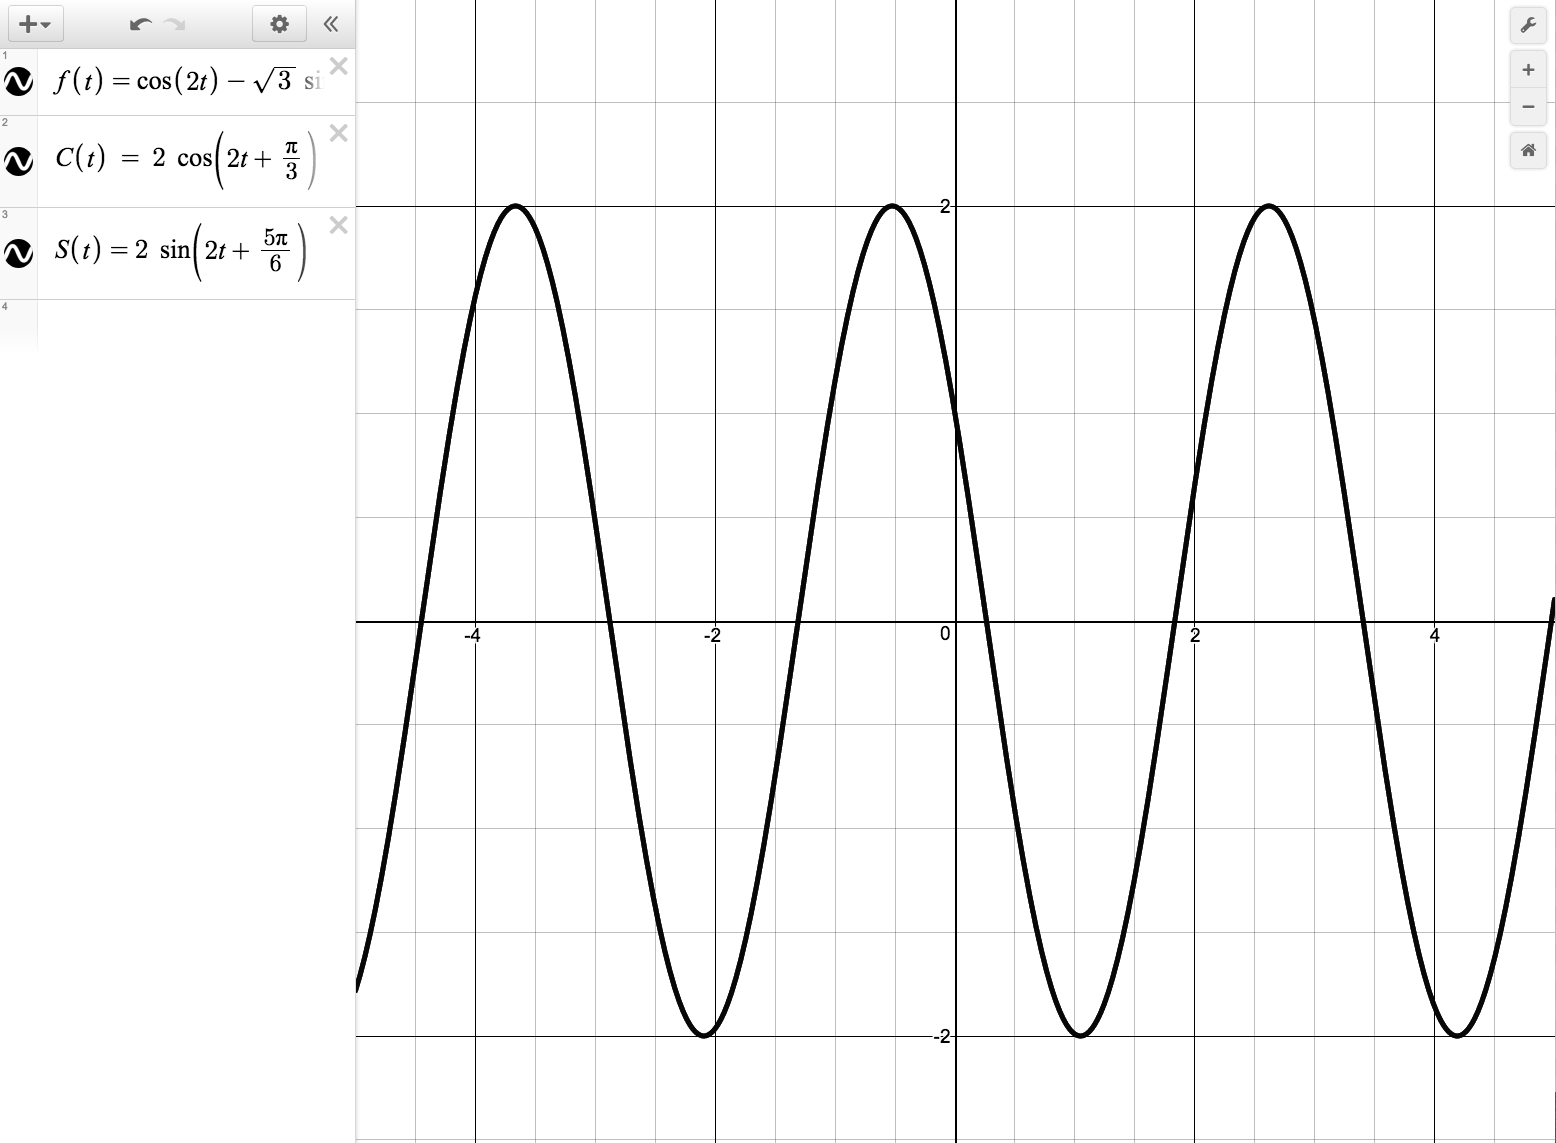
\includegraphics[width=4in]{./MoreTrigonometricIdentitiesGraphics/ExpandedSinusoidExample.jpg} 



\end{center}

\qed

\end{enumerate}

\end{ex}

A couple of remarks about Example \ref{expandedsinusoidex1} are in order.   First, had we chosen  $A = -2$ instead of $A = 2$ as we worked through Example \ref{expandedsinusoidex1}, our final answers would have \textit{looked} different. The reader is encouraged to rework Example  \ref{expandedsinusoidex1} using $A = -2$ to see what these differences are, and then for a challenging exercise, use identities to show that the formulas are all equivalent.\footnote{The general equations to fit a function of the form $f(x) = a \, \cos(\omega x) + b \, \sin(\omega x) + B$ into one of the forms in Theorem \ref{sinusoidform} are explored in Exercise \ref{sinusoidexercise1}.}

\smallskip

It is important to note that in order for the technique presented in Example \ref{expandedsinusoidex1} to fit a function into one of the forms in Theorem \ref{sinusoidform},  the \textit{frequencies} of the sine and cosine terms much match.  For example,  in the Exercises, you'll be asked to write $f(t) = 3\sqrt{3}\sin(3t) - 3\cos(3t)$ in the form of $S(t)$ and $C(t)$ above, and since both the sine and cosine terms have frequency $3$, this is possible.

\smallskip

However, a function such as  $f(t) = \sin(t) - \sin(3t)$ cannot be written in the form of $S(t)$ or $C(t)$. The quickest way to see this is to examine its graph below which is decidedly not a sinusoid.  That being said, we can still analyze this curve using identities.

\phantomsection
\label{beats}

\smallskip


\begin{center}

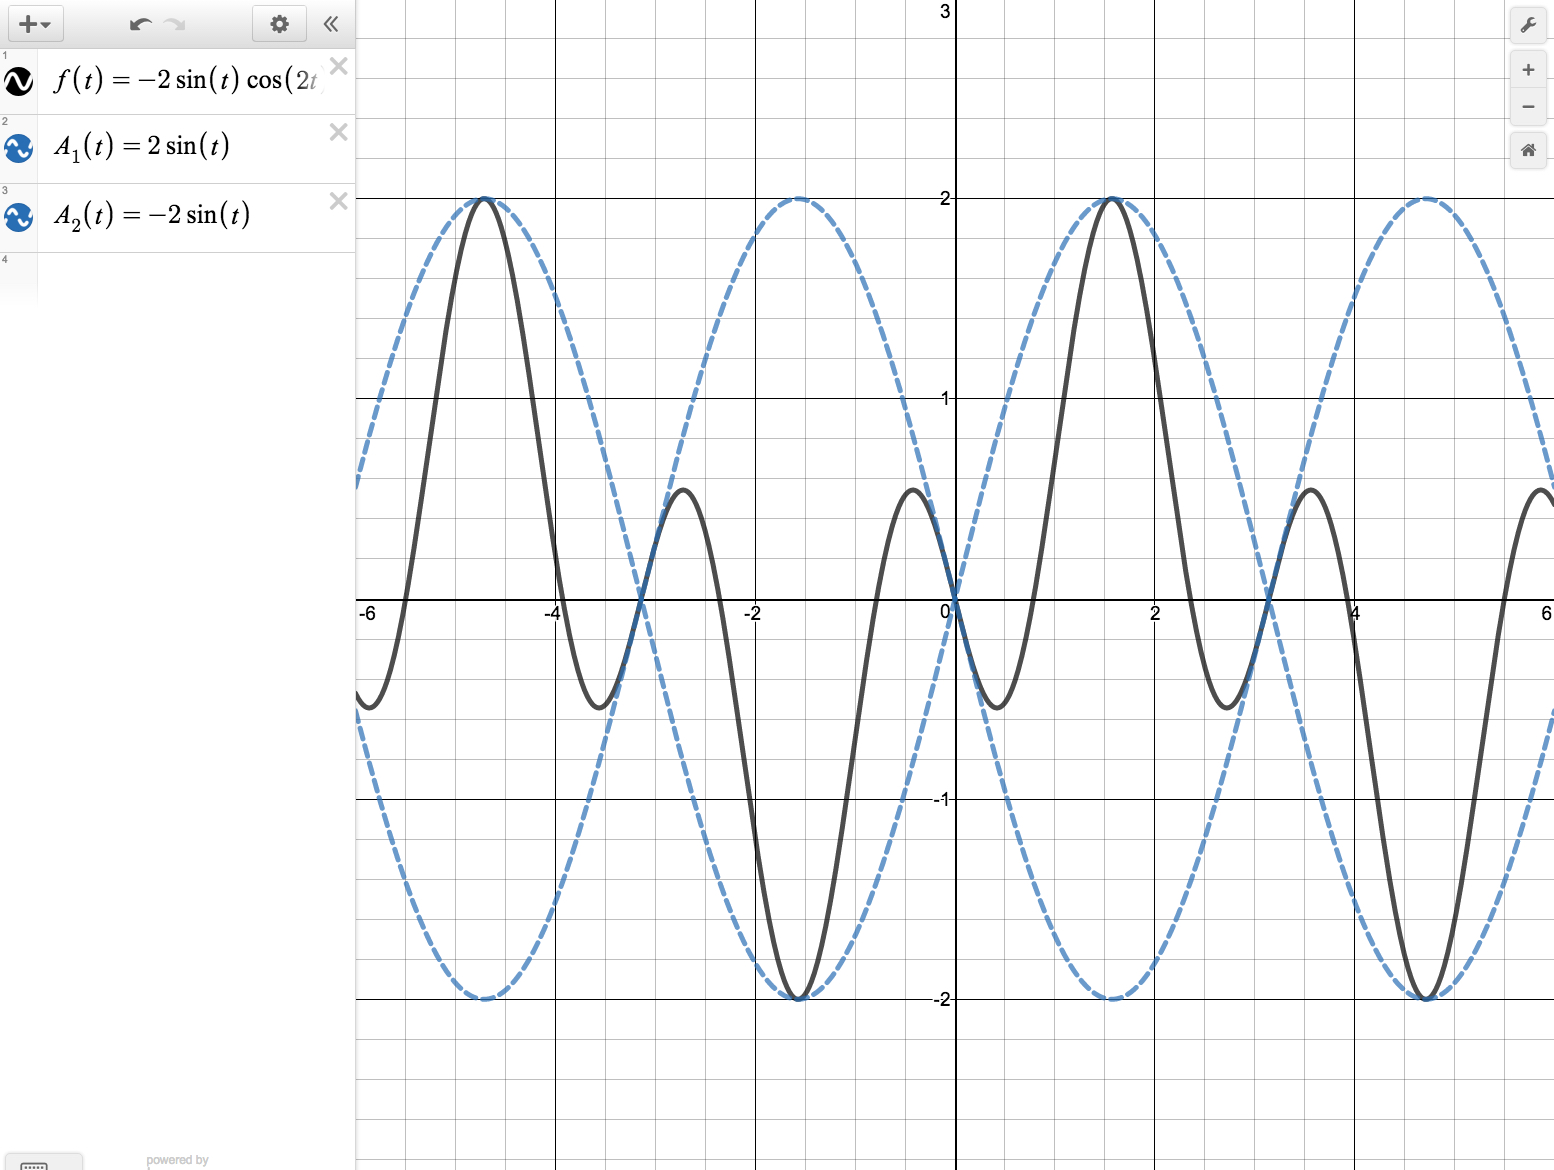
\includegraphics[width=4in]{./MoreTrigonometricIdentitiesGraphics/Beats.jpg} 

\end{center}


 Using our result from  number \ref{beatsprodsumex} Example \ref{prodtosumtoprod}, we may rewrite $f(t) = \sin(t) - \sin(3t) = -2 \sin(t) \cos(2t)$.  Grouping factors, we can view $f(t) = [ -2 \sin(t) ] \cos(2t) = A(t) \cos(2t)$ as the curve $y = \cos(2t)$ with a \textit{variable} amplitude, $A(t) = -2 \sin(t)$. 
 
 \smallskip
 
 Overlaying the graphs of $f(t)$ with the (dashed) graphs of $A_{1}(t) = 2 \sin(t)$ and $A_{2}(t) = -2 \sin(t)$, we can see the role these two curves play in the graph of $y = f(t)$.  They create a kind of `wave envelope' for the graph of $y = f(t)$.  This is an example of the \href{https://en.wikipedia.org/wiki/Beat_(acoustics)}{\underline{beats}} phenomenon.  Note that when written as a product of sinusoids, it is always the \textit{lower} frequency factor which creates the `wave-envelope' of the curve.
 
 \smallskip
 
Note that  in order to rewrite a sum or difference of sine and cosine functions with different frequencies into a product  using the sum to product identities, Theorem \ref{sumtoproduct}, we need the \textit{amplitudes} of each term to be the same.  We explore more examples of these functions and this behavior in the Exercises.
  

\smallskip


\newpage

\subsection{Exercises}

In Exercises \ref{evenoddfirst} - \ref{evenoddlast}, use the Even / Odd Identities to verify the identity.  Assume all quantities are defined.

\begin{multicols}{2}

\begin{enumerate}

\item $\sin(3\pi - 2\theta) = -\sin(2\theta - 3\pi)$ \vphantom{$\left( -\frac{\pi}{4} \right)$} \label{evenoddfirst}
\item $\cos \left( -\frac{\pi}{4} - 5t \right) = \cos \left( 5t + \frac{\pi}{4} \right)$

\setcounter{HW}{\value{enumi}}

\end{enumerate}

\end{multicols}

\begin{multicols}{2}

\begin{enumerate}

\setcounter{enumi}{\value{HW}}

\item $\tan(-x^{2} + 1) = -\tan(x^{2} - 1)$
\item $\csc(-\theta - 5) = -\csc(\theta + 5)$

\setcounter{HW}{\value{enumi}}

\end{enumerate}

\end{multicols}

\begin{multicols}{2}

\begin{enumerate}

\setcounter{enumi}{\value{HW}}

\item $\sec(-6x) = \sec(6x)$
\item $\cot(9 - 7\theta) = -\cot(7\theta - 9)$ \label{evenoddlast}

\setcounter{HW}{\value{enumi}}

\end{enumerate}

\end{multicols}

In Exercises \ref{sumdifffirst} - \ref{sumdifflast}, use the Sum and Difference Identities to find the exact value.  You may have need of the Quotient, Reciprocal or Even / Odd Identities as well.

\begin{multicols}{3}

\begin{enumerate}

\setcounter{enumi}{\value{HW}}

\item  \label{cos75} $\cos(75^{\circ})$ \label{sumdifffirst} 
\item  $\sec(165^{\circ})$
\item  \label{sin105} $\sin(105^{\circ})$

\setcounter{HW}{\value{enumi}}

\end{enumerate}

\end{multicols}

\begin{multicols}{3}

\begin{enumerate}

\setcounter{enumi}{\value{HW}}

\item  $\csc(195^{\circ})$
\item  $\cot(255^{\circ})$
\item  $\tan(375^{\circ})$

\setcounter{HW}{\value{enumi}}

\end{enumerate}

\end{multicols}

\begin{multicols}{3}

\begin{enumerate}

\setcounter{enumi}{\value{HW}}

\item  $\cos\left(\frac{13\pi}{12}\right)$
\item  $\sin\left(\frac{11\pi}{12}\right)$
\item  $\tan\left(\frac{13\pi}{12}\right)$

\setcounter{HW}{\value{enumi}}

\end{enumerate}

\end{multicols}

\begin{multicols}{3}

\begin{enumerate}

\setcounter{enumi}{\value{HW}}

\item \label{cos7pi12} $\cos \left( \frac{7\pi}{12} \right)$
\item $\tan \left( \frac{17\pi}{12} \right)$
\item \label{sinpi12} $\sin \left( \frac{\pi}{12} \right)$ \vphantom{$\left(\frac{13\pi}{12}\right)$}

\setcounter{HW}{\value{enumi}}

\end{enumerate}

\end{multicols}

\begin{multicols}{3}

\begin{enumerate}

\setcounter{enumi}{\value{HW}}

\item $\cot \left( \frac{11\pi}{12} \right)$
\item $\csc \left( \frac{5\pi}{12} \right)$
\item $\sec \left( -\frac{\pi}{12} \right)$ \vphantom{$\left(\frac{13\pi}{12}\right)$} \label{sumdifflast}

\setcounter{HW}{\value{enumi}}

\end{enumerate}

\end{multicols}

\begin{enumerate}

\setcounter{enumi}{\value{HW}}

\item  If $\alpha$ is a Quadrant IV angle with $\cos(\alpha) = \frac{\sqrt{5}}{5}$, and  $\sin(\beta) = \frac{\sqrt{10}}{10}$, where $\frac{\pi}{2} < \beta < \pi$, find

\begin{multicols}{3}

\begin{enumerate}

\item  $\cos(\alpha + \beta)$
\item  $\sin(\alpha + \beta)$
\item  $\tan(\alpha + \beta)$

\setcounter{HWindent}{\value{enumii}}

\end{enumerate}

\end{multicols}

\begin{multicols}{3}

\begin{enumerate}

\setcounter{enumii}{\value{HWindent}}

\item  $\cos(\alpha - \beta)$
\item  $\sin(\alpha - \beta)$
\item  $\tan(\alpha - \beta)$

\end{enumerate}

\end{multicols}

\item  If $\csc(\alpha) = 3$, where $0 < \alpha < \frac{\pi}{2}$, and $\beta$ is a Quadrant II angle with $\tan(\beta) = -7$, find

\begin{multicols}{3}

\begin{enumerate}

\item  $\cos(\alpha + \beta)$
\item  $\sin(\alpha + \beta)$
\item  $\tan(\alpha + \beta)$

\setcounter{HWindent}{\value{enumii}}

\end{enumerate}

\end{multicols}

\begin{multicols}{3}

\begin{enumerate}

\setcounter{enumii}{\value{HWindent}}

\item  $\cos(\alpha - \beta)$
\item  $\sin(\alpha - \beta)$
\item  $\tan(\alpha - \beta)$

\end{enumerate}

\end{multicols}

\item If $\sin(\alpha) = \frac{3}{5}$, where $0 < \alpha < \frac{\pi}{2}$, and $\cos(\beta) = \frac{12}{13}$ where $\frac{3\pi}{2} < \beta < 2\pi$, find 

\begin{multicols}{3}

\begin{enumerate}

\item $\sin(\alpha + \beta)$
\item $\cos(\alpha - \beta)$
\item $\tan(\alpha - \beta)$

\end{enumerate}

\end{multicols}



\item If $\sec(\alpha) = -\frac{5}{3}$, where $\frac{\pi}{2} < \alpha < \pi$, and $\tan(\beta) = \frac{24}{7}$, where $\pi < \beta < \frac{3\pi}{2}$, find

\begin{multicols}{3}

\begin{enumerate}

\item $\csc(\alpha - \beta)$
\item $\sec(\alpha + \beta)$
\item $\cot(\alpha + \beta)$

\end{enumerate}

\end{multicols}

\setcounter{HW}{\value{enumi}}

\end{enumerate}

\newpage

In Exercises \ref{expandedsinusoidexerfirst} - \ref{expandedsinusoidexerlast}, use Example \ref{expandedsinusoidex1} as a guide to show that the function is a sinusoid by rewriting it in the forms $C(t) = A \cos(\omega t + \phi) + B$ and $S(t) = A \sin(\omega t + \phi) + B$ for $\omega > 0$ and $0 \leq \phi < 2\pi$.

\begin{multicols}{2}

\begin{enumerate}

\setcounter{enumi}{\value{HW}}

\item $f(t) = \sqrt{2}\sin(t) + \sqrt{2}\cos(t) + 1$ \label{expandedsinusoidexerfirst}
\item $f(t) = 3\sqrt{3}\sin(3t) - 3\cos(3t)$

\setcounter{HW}{\value{enumi}}

\end{enumerate}

\end{multicols}

\begin{multicols}{2}

\begin{enumerate}

\setcounter{enumi}{\value{HW}}

\item $f(t) = -\sin(t) + \cos(t) - 2$ \vphantom{$\left( -\frac{1\sqrt{3}}{2} \right)$} 
\item $f(t) = -\frac{1}{2}\sin(2t) - \frac{\sqrt{3}}{2}\cos(2t)$

\setcounter{HW}{\value{enumi}}

\end{enumerate}

\end{multicols}

\begin{multicols}{2}

\begin{enumerate}

\setcounter{enumi}{\value{HW}}

\item  $f(t) = 2\sqrt{3} \cos(t) - 2\sin(t)$ \vphantom{$\left( -\frac{3\sqrt{3}}{2} \right)$} 
\item  $f(t) = \frac{3}{2} \cos(2t) - \frac{3\sqrt{3}}{2} \sin(2t) + 6$

\setcounter{HW}{\value{enumi}}

\end{enumerate}

\end{multicols}

\begin{multicols}{2}

\begin{enumerate}

\setcounter{enumi}{\value{HW}}

\item  $f(t) = -\frac{1}{2} \cos(5t) -\frac{\sqrt{3}}{2} \sin(5t)$
\item  $f(t) = -6\sqrt{3} \cos(3t) - 6\sin(3t) - 3$ \vphantom{$\left( -\frac{\sqrt{3}}{2} \right)$} 

\setcounter{HW}{\value{enumi}}

\end{enumerate}

\end{multicols}

\begin{multicols}{2}

\begin{enumerate}

\setcounter{enumi}{\value{HW}}

\item  $f(t) =  \frac{5\sqrt{2}}{2} \sin(t)  -\frac{5\sqrt{2}}{2} \cos(t)$
\item  $f(t) =3 \sin \left(\frac{t}{6}\right) -3\sqrt{3} \cos \left(\frac{t}{6}\right)$ \vphantom{$\left( \frac{-5 \sqrt{3}}{2} \right)$}  \label{expandedsinusoidexerlast}

\setcounter{HW}{\value{enumi}}

\end{enumerate}

\end{multicols}


\begin{enumerate}

\setcounter{enumi}{\value{HW}}

\item In Exercises \ref{expandedsinusoidexerfirst} - \ref{expandedsinusoidexerlast}, you should have noticed a relationship between the phases $\phi$ for the $S(t)$ and $C(t)$.  Show that if $f(t) = A \sin(\omega t + \alpha) + B$, then $f(t) = A \cos(\omega t + \beta) + B$ where $\beta = \alpha - \frac{\pi}{2}$. 
\label{sinusoidexercise1}

\item Let $\phi$ be an angle measured in radians and let $P(a,b)$ be a point on the terminal side of $\phi$ when it is drawn in standard position.  Use Theorem \ref{cosinesinecircle} and the sum identity for sine in Theorem \ref{sinesumdifference} to show that  $f(t) = a \, \sin(\omega t) + b\, \cos(\omega t) + B$ (with  $\omega > 0$) can be rewritten as $f(t) = \sqrt{a^{2} + b^{2}}\sin(\omega t + \phi) + B$.
\label{sinusoidexercise2}

\setcounter{HW}{\value{enumi}}

\end{enumerate}

\begin{enumerate}

\setcounter{enumi}{\value{HW}}

\item  \label{twodaylightfunctions} In Example \ref{sinusoidsunlight} in Section \ref{GraphsofSineandCosine}, we developed two (seemingly) different formulas to model the hours of daylight, $H(t)$:   $H_{1}(t) = 9.25 \sin\left(\frac{\pi}{6} t - \frac{\pi}{2}\right) + 12.55$ and  $H_{2}(t) = -8.13 \sin\left(\frac{\pi}{6} t - 4.70\right)+ 12.5$.  Use the difference identities for sine to expand $H_{1}(t)$ and $H_{2}(t)$.  How different are they?
\setcounter{HW}{\value{enumi}}
\end{enumerate}




In Exercises \ref{identfirstident} - \ref{identlastident}, verify the identity.\footnote{Note: numbers \ref{conversionsineshift} and \ref{conversioncosineshift} are the conversion formulas stated in Theorem \ref{cosinesinefunctionprops} in Section \ref{GraphsofSineandCosine}.}

\begin{multicols}{2}

\begin{enumerate}

\setcounter{enumi}{\value{HW}}

\item  $\sin\left(\theta + \frac{\pi}{2}\right) = \cos(t)$  \label{identfirstident} \label{conversionsineshift}
\item $\cos\left(\theta - \frac{\pi}{2} \right) = \sin(t)$ \label{conversioncosineshift}

\setcounter{HW}{\value{enumi}}

\end{enumerate}

\end{multicols}


\begin{multicols}{2}

\begin{enumerate}

\setcounter{enumi}{\value{HW}}

\item $\cos(\theta - \pi) = -\cos(\theta)$
\item $\sin(\pi - \theta) = \sin(\theta)$

\setcounter{HW}{\value{enumi}}

\end{enumerate}

\end{multicols}

\begin{multicols}{2}

\begin{enumerate}

\setcounter{enumi}{\value{HW}}

\item $\tan\left(\theta + \frac{\pi}{2} \right) = -\cot(\theta)$
\item $\sin(\alpha + \beta) + \sin(\alpha - \beta) = 2\sin(\alpha)\cos(\beta)$ \vphantom{$\left( \frac{\pi}{2} \right)$}

\setcounter{HW}{\value{enumi}}

\end{enumerate}

\end{multicols}

\begin{multicols}{2}

\begin{enumerate}

\setcounter{enumi}{\value{HW}}

\item $\sin(\alpha + \beta) - \sin(\alpha - \beta) = 2\cos(\alpha) \sin(\beta)$
\item $\cos(\alpha + \beta) + \cos(\alpha - \beta) = 2\cos(\alpha) \cos(\beta)$

\setcounter{HW}{\value{enumi}}

\end{enumerate}

\end{multicols}

\begin{multicols}{2}

\begin{enumerate}

\setcounter{enumi}{\value{HW}}

\item $\cos(\alpha + \beta) - \cos(\alpha - \beta) = -2\sin(\alpha) \sin(\beta)$ \vphantom{$\dfrac{\sin(\alpha+\beta)}{\sin(\alpha-\beta)}$}
\item $\dfrac{\sin(\alpha+\beta)}{\sin(\alpha-\beta)} = \dfrac{1+\cot(\alpha) \tan(\beta)}{1 - \cot(\alpha) \tan(\beta)}$ 

\setcounter{HW}{\value{enumi}}

\end{enumerate}

\end{multicols}

\begin{multicols}{2}

\begin{enumerate}

\setcounter{enumi}{\value{HW}}

\item $\dfrac{\cos(\alpha + \beta)}{\cos(\alpha - \beta)} = \dfrac{1 - \tan(\alpha)\tan(\beta)}{1 + \tan(\alpha)\tan(\beta)}$
\item $\dfrac{\tan(\alpha + \beta)}{\tan(\alpha - \beta)} = \dfrac{\sin(\alpha)\cos(\alpha) + \sin(\beta)\cos(\beta)}{\sin(\alpha)\cos(\alpha) - \sin(\beta)\cos(\beta)}$

\setcounter{HW}{\value{enumi}}

\end{enumerate}

\end{multicols}

\begin{enumerate}

\setcounter{enumi}{\value{HW}}

\item $\dfrac{\sin(t + h) - \sin(t)}{h} = \cos(t) \left(\dfrac{\sin(h)}{h} \right) + \sin(t) \left( \dfrac{\cos(h) - 1}{h} \right)$
\item $\dfrac{\cos(t + h) - \cos(t)}{h} = \cos(t) \left( \dfrac{\cos(h) - 1}{h} \right) - \sin(t) \left(\dfrac{\sin(h)}{h} \right)$
\item  $\dfrac{\tan(t + h) - \tan(t)}{h} = \left( \dfrac{\tan(h)}{h} \right) \left(\dfrac{\sec^{2}(t)}{1 - \tan(t)\tan(h)} \right)$ \label{identlastident}

\setcounter{HW}{\value{enumi}}

\end{enumerate}



In Exercises \ref{idenhalfanglefirst} - \ref{idenhalfanglelast}, use the Half Angle Formulas to find the exact value.  You may have need of the Quotient, Reciprocal or Even / Odd Identities as well.

\begin{multicols}{2}

\begin{enumerate}

\setcounter{enumi}{\value{HW}}

\item  $\cos(75^{\circ})$  (compare with Exercise \ref{cos75}) \label{idenhalfanglefirst}
\item  $\sin(105^{\circ})$  (compare with Exercise \ref{sin105})

\setcounter{HW}{\value{enumi}}

\end{enumerate}

\end{multicols}

\begin{multicols}{2}

\begin{enumerate}

\setcounter{enumi}{\value{HW}}

\item  $\cos(67.5^{\circ})$
\item  $\sin(157.5^{\circ})$

\setcounter{HW}{\value{enumi}}

\end{enumerate}

\end{multicols}

\begin{multicols}{2}

\begin{enumerate}

\setcounter{enumi}{\value{HW}}

\item  $\tan(112.5^{\circ})$ \vphantom{$\left( \frac{7\pi}{12} \right)$}
\item  $\cos\left( \frac{7\pi}{12} \right)$  (compare with Exercise \ref{cos7pi12})

\setcounter{HW}{\value{enumi}}

\end{enumerate}

\end{multicols}

\begin{multicols}{2}

\begin{enumerate}

\setcounter{enumi}{\value{HW}}

\item  $\sin\left( \frac{\pi}{12} \right)$  (compare with Exercise \ref{sinpi12})
\item $\cos \left( \frac{\pi}{8} \right)$

\setcounter{HW}{\value{enumi}}

\end{enumerate}

\end{multicols}

\begin{multicols}{2}

\begin{enumerate}

\setcounter{enumi}{\value{HW}}

\item $\sin \left( \frac{5\pi}{8} \right)$
\item $\tan \left( \frac{7\pi}{8} \right)$ \label{idenhalfanglelast}

\setcounter{HW}{\value{enumi}}

\end{enumerate}

\end{multicols}

In Exercises \ref{doublehalffirst} - \ref{doublehalflast}, use the given information about $\theta$ to find the exact values of 

\begin{multicols}{3}

\begin{itemize}

\item $\sin(2\theta)$
\item $\sin\left(\frac{\theta}{2}\right)$
\item $\cos(2\theta)$
\item $\cos\left(\frac{\theta}{2}\right)$
\item $\tan(2\theta)$
\item $\tan\left(\frac{\theta}{2}\right)$

\end{itemize}

\end{multicols}

\begin{multicols}{2}

\begin{enumerate}

\setcounter{enumi}{\value{HW}}

\item $\sin(\theta) = -\frac{7}{25}$ where $\frac{3\pi}{2} < \theta < 2\pi$ \label{doublehalffirst}
\item $\cos(\theta) = \frac{28}{53}$ where $0 < \theta < \frac{\pi}{2}$

\setcounter{HW}{\value{enumi}}

\end{enumerate}

\end{multicols}

\begin{multicols}{2}

\begin{enumerate}

\setcounter{enumi}{\value{HW}}

\item $\tan(\theta) = \frac{12}{5}$ where $\pi < \theta < \frac{3\pi}{2}$
\item $\csc(\theta) = 4$ where $\frac{\pi}{2} < \theta < \pi$

\setcounter{HW}{\value{enumi}}

\end{enumerate}

\end{multicols}

\begin{multicols}{2}

\begin{enumerate}

\setcounter{enumi}{\value{HW}}

\item  $\cos(\theta) = \frac{3}{5}$ where $0 < \theta < \frac{\pi}{2}$
\item  $\sin(\theta) = -\frac{4}{5}$ where $\pi < \theta < \frac{3\pi}{2}$

\setcounter{HW}{\value{enumi}}

\end{enumerate}

\end{multicols}

\begin{multicols}{2}

\begin{enumerate}

\setcounter{enumi}{\value{HW}}

\item  $\cos(\theta) = \frac{12}{13}$ where $\frac{3\pi}{2} < \theta < 2\pi$
\item  $\sin(\theta) = \frac{5}{13}$ where $\frac{\pi}{2} < \theta < \pi$

\setcounter{HW}{\value{enumi}}

\end{enumerate}

\end{multicols}

\begin{multicols}{2}

\begin{enumerate}

\setcounter{enumi}{\value{HW}}

\item  $\sec(\theta) = \sqrt{5}$ where $\frac{3\pi}{2} < \theta < 2\pi$
\item  $\tan(\theta) = -2$ where $\frac{\pi}{2} < \theta < \pi$ \label{doublehalflast}

\setcounter{HW}{\value{enumi}}

\end{enumerate}

\end{multicols}



In Exercises \ref{moreidentfirst} - \ref{moreidentlast}, verify the identity.  Assume all quantities are defined.

\begin{multicols}{2}

\begin{enumerate}

\setcounter{enumi}{\value{HW}}

\item  $(\cos(\theta) + \sin(\theta))^2 = 1 + \sin(2\theta)$ \label{moreidentfirst}
\item  $(\cos(\theta) - \sin(\theta))^2 = 1 - \sin(2\theta)$

\setcounter{HW}{\value{enumi}}

\end{enumerate}

\end{multicols}

\begin{multicols}{2}

\begin{enumerate}

\setcounter{enumi}{\value{HW}}

\item  $\tan(2t) = \frac{1}{1-\tan(t)} - \frac{1}{1+\tan(t)}$
\item  $\csc(2\theta) = \frac{\cot(\theta) + \tan(\theta)}{2}$

\setcounter{HW}{\value{enumi}}

\end{enumerate}

\end{multicols}

\begin{multicols}{2}

\begin{enumerate}

\setcounter{enumi}{\value{HW}}

\item  $8 \sin^{4}(x) = \cos(4x) - 4\cos(2x)+3$
\item  $8 \cos^{4}(x) = \cos(4x) + 4\cos(2x)+3$

\setcounter{HW}{\value{enumi}}

\end{enumerate}

\end{multicols}

\begin{multicols}{2}

\begin{enumerate}

\setcounter{enumi}{\value{HW}}

\item \label{sine3theta} $\sin(3\theta) = 3\sin(\theta) - 4\sin^{3}(\theta)$
\item  $\sin(4\theta) = 4\sin(\theta)\cos^{3}(\theta) - 4\sin^{3}(\theta)\cos(\theta)$

\setcounter{HW}{\value{enumi}}

\end{enumerate}

\end{multicols}

\begin{enumerate}

\setcounter{enumi}{\value{HW}}

\item  $32\sin^{2}(t) \cos^{4}(t) = 2 + \cos(2t) - 2\cos(4t) - \cos(6t)$
\item  $32\sin^{4}(t) \cos^{2}(t) = 2 - \cos(2t) - 2\cos(4t) + \cos(6t)$
\item \label{cosine4theta} $\cos(4\theta) = 8\cos^{4}(\theta) - 8\cos^{2}(\theta) + 1$
\item  $\cos(8\theta) = 128\cos^{8}(\theta)-256\cos^{6}(\theta)+160\cos^{4}(\theta)-32\cos^{2}(\theta)+1$ (HINT:  Use the result to \ref{cosine4theta}.)
\item  $\sec(2x) = \dfrac{\cos(x)}{\cos(x) + \sin(x)} + \dfrac{\sin(x)}{\cos(x)-\sin(x)}$ 
\item  $\dfrac{1}{\cos(\theta) - \sin(\theta)} + \dfrac{1}{\cos(\theta) + \sin(\theta)} = \dfrac{2\cos(\theta)}{\cos(2\theta)}$
\item  $\dfrac{1}{\cos(\theta) - \sin(\theta)} - \dfrac{1}{\cos(\theta) + \sin(\theta)} = \dfrac{2\sin(\theta)}{\cos(2\theta)}$ \label{moreidentlast}

\setcounter{HW}{\value{enumi}}

\end{enumerate}

\begin{enumerate}

\setcounter{enumi}{\value{HW}}

\item  \label{preludetoarctrigsine} Suppose $\theta$ is a Quadrant I angle with $\sin(\theta) = x$. Verify the following formulas

\begin{multicols}{3}

\begin{enumerate}

\item  $\cos(\theta) = \sqrt{1-x^2}$

\item  $\sin(2\theta) = 2x\sqrt{1-x^2}$

\item $\cos(2\theta) = 1 - 2x^2$

\end{enumerate}

\end{multicols}

\item  Discuss with your classmates how each of the formulas, if any, in Exercise \ref{preludetoarctrigsine} change if we change assume $\theta$ is a Quadrant II, III, or IV angle.

\item  \label{preludetoarctrigtan} Suppose $\theta$ is a Quadrant I angle with $\tan(\theta) = x$. Verify the following formulas

\begin{multicols}{2}

\begin{enumerate}

\item $\cos(\theta) = \dfrac{1}{\sqrt{x^2+1}}$
\item $\sin(\theta) = \dfrac{x}{\sqrt{x^2+1}}$

\setcounter{HWindent}{\value{enumii}}

\end{enumerate}

\end{multicols}

\begin{multicols}{2}

\begin{enumerate}

\setcounter{enumii}{\value{HWindent}}

\item $\sin(2\theta) = \dfrac{2x}{x^2+1}$
\item $\cos(2\theta) = \dfrac{1-x^2}{x^2+1}$

\end{enumerate}

\end{multicols}

\item  Discuss with your classmates how each of the formulas, if any, in Exercise \ref{preludetoarctrigtan} change if we change assume $\theta$ is a Quadrant II, III, or IV angle.

\item  If $\sin(t) = x$ for  $-\frac{\pi}{2} < t < \frac{\pi}{2}$, find an expression for $\tan(t)$ in terms of $x$.

\item  If $\tan(\theta) = x$ for $-\frac{\pi}{2} < \theta < \frac{\pi}{2}$,  find an expression for $\sec(\theta)$ in terms of $x$.

\item  If $\sec(\theta) = x$ where  $\theta$ is a Quadrant II angle, find  an expression for $\tan(\theta)$ in terns of $x$.

\item If $\sin(t) = \frac{x}{2}$ for $-\frac{\pi}{2} < t < \frac{\pi}{2}$, find an expression for $\cos(2t)$ in terms of $x$.

\item If $\tan(\theta) = \frac{x}{7}$ for $-\frac{\pi}{2} < \theta < \frac{\pi}{2}$, find an expression for $\sin(2\theta)$ in terms of $x$.

\item If $\sec(t) = \frac{x}{4}$ for $0 < t < \frac{\pi}{2}$, find an expression for $\ln|\sec(t) + \tan(t)|$ in terms of $x$.

\item Show that $\cos^{2}(\theta) - \sin^{2}(\theta) = 2\cos^{2}(\theta) - 1 = 1 - 2\sin^{2}(\theta)$ for all $\theta$.

\item Let $\theta$ be a Quadrant III angle with $\cos(\theta) = -\frac{1}{5}$.  Show that this is not enough information to determine the sign of  $\sin\left(\frac{\theta}{2}\right)$ by first assuming $3\pi < \theta < \frac{7\pi}{2}$ and then assuming $\pi < \theta < \frac{3\pi}{2}$ and computing $\sin\left(\frac{\theta}{2}\right)$ in both cases.

\item Without using your calculator, show that $\frac{\sqrt{2 + \sqrt{3}}}{2} = \frac{\sqrt{6} + \sqrt{2}}{4}$

\item In part \ref{cosinepolynomial} of Example \ref{doubleangleex}, we wrote $\cos(3\theta)$ as a polynomial in terms of $\cos(\theta)$.  In Exercise \ref{cosine4theta}, we had you verify an identity which expresses $\cos(4\theta)$ as a polynomial in terms of $\cos(\theta)$.   Can you find a polynomial in terms of $\cos(\theta)$ for $\cos(5\theta)$?  $\cos(6\theta)$?  Can you find a pattern so that $\cos(n\theta)$ could be written as a polynomial in cosine for any natural number $n$?

\item In Exercise \ref{sine3theta}, we has you verify an identity which expresses $\sin(3\theta)$ as a polynomial in terms of $\sin(\theta)$.   Can you do the same for  $\sin(5\theta)$?  What about for $\sin(4\theta)$?  If not, what goes wrong?

\setcounter{HW}{\value{enumi}}

\end{enumerate}

In Exercises \ref{idengraphfirst} - \ref{idengraphlast}, verify the identity by graphing the right and left hand using a graphing utility.

\begin{multicols}{3}

\begin{enumerate}

\setcounter{enumi}{\value{HW}}

\item $\sin^{2}(t) + \cos^{2}(t) = 1$ \vphantom{$\left( \frac{\pi}{2} \right)$} \label{idengraphfirst} 
\item $\sec^{2}(x) - \tan^{2}(x) = 1$ \vphantom{$\left( \frac{\pi}{2} \right)$}
\item  $\cos(t) = \sin\left(\frac{\pi}{2} - t\right)$

\setcounter{HW}{\value{enumi}}

\end{enumerate}

\end{multicols}

\begin{multicols}{3}

\begin{enumerate}

\setcounter{enumi}{\value{HW}}

\item  $\tan(x+\pi) = \tan(x)$ \vphantom{$\frac{\sin(x)}{1+\cos(x)}$}
\item  $\sin(2t) = 2\sin(t)\cos(t)$ \vphantom{$\frac{\sin(x)}{1+\cos(x)}$}
\item  $\tan\left(\frac{x}{2}\right) = \frac{\sin(x)}{1+\cos(x)}$ \label{idengraphlast}

\setcounter{HW}{\value{enumi}}

\end{enumerate}

\end{multicols}


In Exercises \ref{prodsumfirst} - \ref{prodsumlast}, write the  given product as a sum. Note: you may need to use an Even/Odd Identity to match the answer provided.

\begin{multicols}{3}

\begin{enumerate}

\setcounter{enumi}{\value{HW}}

\item $\cos(3\theta)\cos(5\theta)$ \label{prodsumfirst}
\item $\sin(2t)\sin(7t)$
\item $\sin(9x)\cos(x)$

\setcounter{HW}{\value{enumi}}

\end{enumerate}

\end{multicols}

\begin{multicols}{3}

\begin{enumerate}

\setcounter{enumi}{\value{HW}}

\item $\cos(2\theta) \cos(6\theta)$
\item $\sin(3t) \sin(2t)$
\item $\cos(x) \sin(3x)$ \label{prodsumlast}

\setcounter{HW}{\value{enumi}}

\end{enumerate}

\end{multicols}

In Exercises \ref{sumprodfirst} - \ref{sumprodlast},  write the given sum as a product. Note:  you may need to use an Even/Odd or Cofunction Identity to match the answer provided.

\begin{multicols}{3}

\begin{enumerate}

\setcounter{enumi}{\value{HW}}

\item $\cos(3\theta) + \cos(5\theta)$ \label{sumprodfirst}
\item $\sin(2t) - \sin(7t)$
\item $\cos(5x) - \cos(6x)$

\setcounter{HW}{\value{enumi}}

\end{enumerate}

\end{multicols}

\begin{multicols}{3}

\begin{enumerate}

\setcounter{enumi}{\value{HW}}

\item $\sin(9\theta) - \sin(-\theta)$
\item $\sin(t) + \cos(t)$
\item $\cos(x) - \sin(x)$ \label{sumprodlast}

\setcounter{HW}{\value{enumi}}

\end{enumerate}

\end{multicols}


In Exercises \ref{beatexfirst} - \ref{beatexlast}, using the remarks following Example \ref{expandedsinusoidex1} on page \pageref{beats} as a guide,  rewrite the given function $f(t)$ as a product of sinusoids. Identify the functions which create the `wave envelope.' Check your answer by graphing  the function along with the `wave-envelope' using a graphing utility.

\begin{multicols}{2}

\begin{enumerate}

\setcounter{enumi}{\value{HW}}

\item $f(t) = \cos(3t) + \cos(5t)$ \label{beatexfirst}
\item $f(t) = 3\cos(5t) - 3\cos(6t)$
\setcounter{HW}{\value{enumi}}

\end{enumerate}

\end{multicols}

\begin{multicols}{2}

\begin{enumerate}

\setcounter{enumi}{\value{HW}}

\item $f(t) = \frac{1}{2} \sin(9t) + \frac{1}{2} \sin(t)$
\item $f(t) = \frac{2}{3}\sin(2t) - \frac{2}{3}\sin(7t)$\label{beatexlast}

\setcounter{HW}{\value{enumi}}

\end{enumerate}

\end{multicols}

\begin{enumerate}

\setcounter{enumi}{\value{HW}}

\item Verify the Even / Odd Identities for tangent, secant, cosecant and cotangent.

\item Verify the Cofunction Identities for tangent, secant, cosecant and cotangent.

\item Verify the Difference Identities for sine and tangent.

\item Verify the Product to Sum Identities.

\item Verify the Sum to Product Identities.

\end{enumerate}

\newpage

\subsection{Answers}

\begin{multicols}{2}

\begin{enumerate}

\addtocounter{enumi}{6}

\item  $\cos(75^{\circ}) = \frac{\sqrt{6} - \sqrt{2}}{4} $
\item  $\sec(165^{\circ}) = -\frac{4}{\sqrt{2}+\sqrt{6}} = \sqrt{2} - \sqrt{6}$

\setcounter{HW}{\value{enumi}}

\end{enumerate}

\end{multicols}

\begin{multicols}{2}

\begin{enumerate}

\setcounter{enumi}{\value{HW}}

\item  $\sin(105^{\circ}) = \frac{\sqrt{6}+\sqrt{2}}{4}$
\item  $\csc(195^{\circ}) = \frac{4}{\sqrt{2}-\sqrt{6}} = -(\sqrt{2}+\sqrt{6})$

\setcounter{HW}{\value{enumi}}

\end{enumerate}

\end{multicols}

\begin{multicols}{2}

\begin{enumerate}

\setcounter{enumi}{\value{HW}}

\item  $\cot(255^{\circ}) = \frac{\sqrt{3}-1}{\sqrt{3}+1} = 2-\sqrt{3}$
\item  $\tan(375^{\circ}) = \frac{3-\sqrt{3}}{3+\sqrt{3}} = 2-\sqrt{3}$

\setcounter{HW}{\value{enumi}}

\end{enumerate}

\end{multicols}

\begin{multicols}{2}

\begin{enumerate}

\setcounter{enumi}{\value{HW}}

\item  $\cos\left(\frac{13\pi}{12}\right) = -\frac{\sqrt{6}+\sqrt{2}}{4}$
\item  $\sin\left(\frac{11\pi}{12}\right) = \frac{\sqrt{6} - \sqrt{2}}{4}$

\setcounter{HW}{\value{enumi}}

\end{enumerate}

\end{multicols}

\begin{multicols}{2}

\begin{enumerate}

\setcounter{enumi}{\value{HW}}

\item  $\tan\left(\frac{13\pi}{12}\right) = \frac{3-\sqrt{3}}{3+\sqrt{3}} = 2-\sqrt{3}$
\item $\cos \left( \frac{7\pi}{12} \right) = \frac{\sqrt{2} - \sqrt{6}}{4}$

\setcounter{HW}{\value{enumi}}

\end{enumerate}

\end{multicols}

\begin{multicols}{2}

\begin{enumerate}

\setcounter{enumi}{\value{HW}}

\item $\tan \left( \frac{17\pi}{12} \right) = 2 + \sqrt{3}$
\item $\sin \left( \frac{\pi}{12} \right) = \frac{\sqrt{6} - \sqrt{2}}{4}$

\setcounter{HW}{\value{enumi}}

\end{enumerate}

\end{multicols}

\begin{multicols}{2}

\begin{enumerate}

\setcounter{enumi}{\value{HW}}

\item $\cot \left( \frac{11\pi}{12} \right) = -(2 + \sqrt{3})$
\item $\csc \left( \frac{5\pi}{12} \right) = \sqrt{6} - \sqrt{2}$

\setcounter{HW}{\value{enumi}}

\end{enumerate}

\end{multicols}

\begin{multicols}{2}

\begin{enumerate}

\setcounter{enumi}{\value{HW}}

\item $\sec \left( -\frac{\pi}{12} \right) = \sqrt{6} - \sqrt{2}$

\setcounter{HW}{\value{enumi}}

\end{enumerate}

\end{multicols}

\begin{enumerate}

\setcounter{enumi}{\value{HW}}

\item \begin{multicols}{2}

\begin{enumerate}

\item  $\cos(\alpha + \beta) = -\frac{\sqrt{2}}{10}$
\item  $\sin(\alpha + \beta) = \frac{7\sqrt{2}}{10}$

\setcounter{HWindent}{\value{enumii}}

\end{enumerate}

\end{multicols}

\begin{multicols}{2}

\begin{enumerate}

\setcounter{enumii}{\value{HWindent}}

\item  $\tan(\alpha + \beta) = -7$ \vphantom{$\frac{\sqrt{2}}{2}$}
\item  $\cos(\alpha - \beta)= -\frac{\sqrt{2}}{2}$

\setcounter{HWindent}{\value{enumii}}

\end{enumerate}

\end{multicols}

\begin{multicols}{2}

\begin{enumerate}

\setcounter{enumii}{\value{HWindent}}

\item  $\sin(\alpha - \beta) = \frac{\sqrt{2}}{2}$
\item  $\tan(\alpha - \beta) = -1$ \vphantom{$\frac{\sqrt{2}}{2}$}

\end{enumerate}

\end{multicols}

\item \begin{multicols}{2}

\begin{enumerate}

\item  $\cos(\alpha + \beta) = - \frac{4+7\sqrt{2}}{30}$
\item  $\sin(\alpha + \beta) = \frac{28-\sqrt{2}}{30}$

\setcounter{HWindent}{\value{enumii}}

\end{enumerate}

\end{multicols}

\begin{multicols}{2}

\begin{enumerate}

\setcounter{enumii}{\value{HWindent}}

\item  $\tan(\alpha + \beta) = \frac{-28+\sqrt{2}}{4+7\sqrt{2}} = \frac{63-100\sqrt{2}}{41}$
\item  $\cos(\alpha - \beta) =  \frac{-4+7\sqrt{2}}{30}$

\setcounter{HWindent}{\value{enumii}}

\end{enumerate}

\end{multicols}

\begin{multicols}{2}

\begin{enumerate}

\setcounter{enumii}{\value{HWindent}}

\item  $\sin(\alpha - \beta) = - \frac{28+\sqrt{2}}{30}$
\item  $\tan(\alpha - \beta)= \frac{28+\sqrt{2}}{4-7\sqrt{2}} = -\frac{63+100\sqrt{2}}{41}$

\end{enumerate}

\end{multicols}

\item \begin{multicols}{3}

\begin{enumerate}

\item $\sin(\alpha + \beta) = \frac{16}{65}$
\item $\cos(\alpha - \beta) = \frac{33}{65}$
\item $\tan(\alpha - \beta) = \frac{56}{33}$

\end{enumerate}

\end{multicols}

 

\item \begin{multicols}{3}

\begin{enumerate}

\item $\csc(\alpha - \beta) = -\frac{5}{4}$
\item $\sec(\alpha + \beta) = \frac{125}{117}$
\item $\cot(\alpha + \beta) = \frac{117}{44}$

\end{enumerate}

\end{multicols}

\setcounter{HW}{\value{enumi}}

\end{enumerate}

\begin{enumerate}
\setcounter{enumi}{\value{HW}}
\item $f(t) = \sqrt{2}\sin(t) + \sqrt{2}\cos(t) + 1 = 2\sin\left(t + \frac{\pi}{4}\right) + 1 = 2\cos\left(t + \frac{7\pi}{4}\right) + 1$ 
\item $f(t) = 3\sqrt{3}\sin(3t) - 3\cos(3t) = 6\sin\left(3t + \frac{11\pi}{6}\right) = 6\cos\left(3t + \frac{4\pi}{3}\right)$
\item $f(t) = -\sin(t) + \cos(t) - 2 = \sqrt{2}\sin\left(t + \frac{3\pi}{4}\right) - 2 = \sqrt{2}\cos\left(t + \frac{\pi}{4}\right) - 2$
\item $f(t) = -\frac{1}{2}\sin(2t) - \frac{\sqrt{3}}{2}\cos(2t) = \sin\left(2t + \frac{4\pi}{3}\right) = \cos\left(2t + \frac{5\pi}{6}\right)$
\item $f(t) = 2\sqrt{3} \cos(t) - 2\sin(t) = 4\sin\left(t+\frac{2\pi}{3}  \right)  = 4\cos\left(t + \frac{\pi}{6}\right)$
\item  $f(t) = \frac{3}{2} \cos(2t) - \frac{3\sqrt{3}}{2} \sin(2t) + 6 =3\sin\left(2t + \frac{5\pi}{6}\right) + 6   = 3\cos\left(2t + \frac{\pi}{3}\right) + 6$
\item  $f(t) = -\frac{1}{2} \cos(5t) -\frac{\sqrt{3}}{2} \sin(5t) =  \sin\left(5t + \frac{7\pi}{6}\right) = \cos\left(5t + \frac{2\pi}{3}\right)$
\item  $f(t) = -6\sqrt{3} \cos(3t) - 6\sin(3t) - 3 = 12\sin\left(3t + \frac{4\pi}{3}\right) - 3 = 12\cos\left(3t + \frac{5\pi}{6}\right) - 3$
\item  $f(t) =  \frac{5\sqrt{2}}{2} \sin(t)  -\frac{5\sqrt{2}}{2} \cos(t) = 5\sin\left(t + \frac{7\pi}{4}\right)= 5\cos\left(t + \frac{5\pi}{4}\right)$
\item  $f(t) =3\sin\left(\frac{t}{6}\right) -3\sqrt{3} \cos\left(\frac{t}{6}\right) = 6\sin\left( \frac{t}{6}+\frac{5\pi}{3}\right)= 6\cos\left( \frac{t}{6}+\frac{7\pi}{6}\right) $

\setcounter{HW}{\value{enumi}}
\end{enumerate}

\begin{multicols}{2}

\begin{enumerate}

\setcounter{enumi}{\value{HW}}

\addtocounter{enumi}{18}

\item $\cos(75^{\circ}) = \frac{\sqrt{2-\sqrt{3}}}{2}$ 
\item $\sin(105^{\circ}) = \frac{\sqrt{2+\sqrt{3}}}{2}$ 

\setcounter{HW}{\value{enumi}}

\end{enumerate}

\end{multicols}

\begin{multicols}{2}

\begin{enumerate}

\setcounter{enumi}{\value{HW}}

\item $\cos(67.5^{\circ})  = \frac{\sqrt{2-\sqrt{2}}}{2}$ 
\item $\sin(157.5^{\circ}) = \frac{\sqrt{2-\sqrt{2}}}{2}$ 

\setcounter{HW}{\value{enumi}}

\end{enumerate}

\end{multicols}

\begin{multicols}{2}

\begin{enumerate}

\setcounter{enumi}{\value{HW}}

\item $\tan(112.5^{\circ}) = - \sqrt{\frac{2+\sqrt{2}}{2-\sqrt{2}}} = -1 - \sqrt{2}$
\item $\cos\left( \frac{7\pi}{12} \right) = -\frac{\sqrt{2-\sqrt{3}}}{2}$  

\setcounter{HW}{\value{enumi}}

\end{enumerate}

\end{multicols}

\begin{multicols}{2}

\begin{enumerate}

\setcounter{enumi}{\value{HW}}

\item $\sin\left( \frac{\pi}{12} \right) = \frac{\sqrt{2-\sqrt{3}}}{2}$ 
\item $\cos \left( \frac{\pi}{8} \right) = \frac{\sqrt{2 + \sqrt{2}}}{2}$

\setcounter{HW}{\value{enumi}}

\end{enumerate}

\end{multicols}

\begin{multicols}{2}

\begin{enumerate}

\setcounter{enumi}{\value{HW}}

\item $\sin \left( \frac{5\pi}{8} \right) = \frac{\sqrt{2 + \sqrt{2}}}{2}$
\item $\tan \left( \frac{7\pi}{8} \right) = -\sqrt{ \frac{2 - \sqrt{2}}{2 + \sqrt{2}} } =1-\sqrt{2}$

\setcounter{HW}{\value{enumi}}

\end{enumerate}

\end{multicols}

\begin{enumerate}

\setcounter{enumi}{\value{HW}}

\item \begin{multicols}{3}

\begin{itemize}

\item $\sin(2\theta) = -\frac{336}{625}$
\item $\sin\left(\frac{\theta}{2}\right) = \frac{\sqrt{2}}{10}$
\item $\cos(2\theta) = \frac{527}{625}$
\item $\cos\left(\frac{\theta}{2}\right) = -\frac{7\sqrt{2}}{10}$
\item $\tan(2\theta) = -\frac{336}{527}$
\item $\tan\left(\frac{\theta}{2}\right) = -\frac{1}{7}$

\end{itemize}

\end{multicols}

\item \begin{multicols}{3}

\begin{itemize}

\item $\sin(2\theta) = \frac{2520}{2809}$
\item $\sin\left(\frac{\theta}{2}\right) = \frac{5\sqrt{106}}{106}$
\item $\cos(2\theta) = -\frac{1241}{2809}$
\item $\cos\left(\frac{\theta}{2}\right) = \frac{9\sqrt{106}}{106}$
\item $\tan(2\theta) = -\frac{2520}{1241}$
\item $\tan\left(\frac{\theta}{2}\right) = \frac{5}{9}$

\end{itemize}

\end{multicols}

\item \begin{multicols}{3}

\begin{itemize}

\item $\sin(2\theta) = \frac{120}{169}$
\item $\sin\left(\frac{\theta}{2}\right) = \frac{3\sqrt{13}}{13}$
\item $\cos(2\theta) = -\frac{119}{169}$
\item $\cos\left(\frac{\theta}{2}\right) = -\frac{2\sqrt{13}}{13}$
\item $\tan(2\theta) = -\frac{120}{119}$
\item $\tan\left(\frac{\theta}{2}\right) = -\frac{3}{2}$

\end{itemize}

\end{multicols}

\item \begin{multicols}{3}

\begin{itemize}

\item $\sin(2\theta) = -\frac{\sqrt{15}}{8}$
\item $\sin\left(\frac{\theta}{2}\right) =\frac{\sqrt{8+2\sqrt{15}}}{4} \\ \phantom{\tan\left(\frac{\theta}{2}\right) = 4+\sqrt{15}}$ 
\item $\cos(2\theta) = \frac{7}{8}$
\item $\cos\left(\frac{\theta}{2}\right) = \frac{\sqrt{8-2\sqrt{15}}}{4} \\ \phantom{\tan\left(\frac{\theta}{2}\right) = 4+\sqrt{15}} $
\item $\tan(2\theta) = -\frac{\sqrt{15}}{7}$
\item $\tan\left(\frac{\theta}{2}\right) = \sqrt{\frac{8+2\sqrt{15}}{8-2\sqrt{15}}} \\ \tan\left(\frac{\theta}{2}\right) = 4+\sqrt{15}$

\end{itemize}

\end{multicols}

\item \begin{multicols}{3}

\begin{itemize}

\item $\sin(2\theta) = \frac{24}{25}$
\item $\sin\left(\frac{\theta}{2}\right) = \frac{\sqrt{5}}{5}$
\item $\cos(2\theta) = -\frac{7}{25}$
\item $\cos\left(\frac{\theta}{2}\right) = \frac{2\sqrt{5}}{5}$
\item $\tan(2\theta)=-\frac{24}{7} $
\item $\tan\left(\frac{\theta}{2}\right) = \frac{1}{2}$

\end{itemize}

\end{multicols}



\item \begin{multicols}{3}

\begin{itemize}

\item $\sin(2\theta) = \frac{24}{25}$
\item $\sin\left(\frac{\theta}{2}\right) = \frac{2\sqrt{5}}{5}$
\item $\cos(2\theta) = -\frac{7}{25}$
\item $\cos\left(\frac{\theta}{2}\right) = -\frac{\sqrt{5}}{5}$
\item $\tan(2\theta)=-\frac{24}{7} $
\item $\tan\left(\frac{\theta}{2}\right) = -2$

\end{itemize}

\end{multicols}

\item \begin{multicols}{3}

\begin{itemize}

\item $\sin(2\theta) = -\frac{120}{169}$
\item $\sin\left(\frac{\theta}{2}\right) = \frac{\sqrt{26}}{26}$
\item $\cos(2\theta) = \frac{119}{169}$
\item $\cos\left(\frac{\theta}{2}\right) = -\frac{5\sqrt{26}}{26}$
\item $\tan(2\theta)=-\frac{120}{119}$
\item $\tan\left(\frac{\theta}{2}\right) = -\frac{1}{5}$

\end{itemize}

\end{multicols}

\item \begin{multicols}{3}

\begin{itemize}

\item $\sin(2\theta) = -\frac{120}{169}$
\item $\sin\left(\frac{\theta}{2}\right) = \frac{5\sqrt{26}}{26}$
\item $\cos(2\theta) = \frac{119}{169}$
\item $\cos\left(\frac{\theta}{2}\right) = \frac{\sqrt{26}}{26}$
\item $\tan(2\theta)=-\frac{120}{119}$
\item $\tan\left(\frac{\theta}{2}\right) = 5$

\end{itemize}

\end{multicols}

\item \begin{multicols}{3}

\begin{itemize}

\item $\sin(2\theta) = -\frac{4}{5}$
\item $\sin\left(\frac{\theta}{2}\right) = \frac{\sqrt{50-10\sqrt{5}}}{10} \\ \phantom{\tan\left(\frac{\theta}{2}\right) =\frac{5-5\sqrt{5}}{10}}$ 

\item $\cos(2\theta) = -\frac{3}{5}$
\item $\cos\left(\frac{\theta}{2}\right)= -\frac{\sqrt{50+10\sqrt{5}}}{10} \\ \phantom{\tan\left(\frac{\theta}{2}\right) =\frac{5-5\sqrt{5}}{10}}$ 
\item $\tan(2\theta)=\frac{4}{3}$
\item $\tan\left(\frac{\theta}{2}\right) =  -\sqrt{\frac{5-\sqrt{5}}{5+\sqrt{5}}} \\ \tan\left(\frac{\theta}{2}\right) =\frac{5-5\sqrt{5}}{10}$

\end{itemize}

\end{multicols}

\item \begin{multicols}{3}

\begin{itemize}

\item $\sin(2\theta) = -\frac{4}{5}$
\item $\sin\left(\frac{\theta}{2}\right) = \frac{\sqrt{50+10\sqrt{5}}}{10} \\ \phantom{\tan\left(\frac{\theta}{2}\right) =\frac{5-5\sqrt{5}}{10}}$ 

\item $\cos(2\theta) = -\frac{3}{5}$
\item $\cos\left(\frac{\theta}{2}\right)= \frac{\sqrt{50-10\sqrt{5}}}{10} \\ \phantom{\tan\left(\frac{\theta}{2}\right) =\frac{5-5\sqrt{5}}{10}}$ 
\item $\tan(2\theta)=\frac{4}{3}$
\item $\tan\left(\frac{\theta}{2}\right) =  \sqrt{\frac{5+\sqrt{5}}{5-\sqrt{5}}} \\ \tan\left(\frac{\theta}{2}\right) =\frac{5+5\sqrt{5}}{10}$

\end{itemize}

\end{multicols}

\setcounter{HW}{\value{enumi}}

\end{enumerate}

\begin{multicols}{3}
\begin{enumerate}
\setcounter{enumi}{\value{HW}}

\addtocounter{enumi}{19}

\item  $\tan(t) = \frac{x}{\sqrt{1 - x^2}}$

\item  $\sec(\theta) = \sqrt{1+x^2}$ \vphantom{$\tan(\theta) = \frac{x}{\sqrt{1 - x^2}}$}

\item  $\tan(\theta) = -\sqrt{x^2-1}$ \vphantom{$\tan(\theta) = \frac{x}{\sqrt{1 - x^2}}$}

\setcounter{HW}{\value{enumi}}
\end{enumerate}

\end{multicols}

\begin{multicols}{2}
\begin{enumerate}

\setcounter{enumi}{\value{HW}}

\item $\cos(2t) = 1 - \dfrac{x^{2}}{2}$

\item $\sin(2\theta) = \dfrac{14x}{x^{2} + 49}$

\setcounter{HW}{\value{enumi}}

\end{enumerate}

\end{multicols}

\begin{enumerate}

\setcounter{enumi}{\value{HW}}
\item $\ln|\sec(t) + \tan(t)| = \ln |x + \sqrt{x^{2} + 16}| - \ln(4)$ \vphantom{$\frac{14x}{x^{2} + 49}$}

\setcounter{HW}{\value{enumi}}

\end{enumerate}

\begin{multicols}{3}

\begin{enumerate}

\setcounter{enumi}{\value{HW}}

\addtocounter{enumi}{11}

\item $\dfrac{\cos(2\theta) + \cos(8\theta)}{2}$
\item $\dfrac{\cos(5t) - \cos(9t)}{2}$
\item $\dfrac{\sin(8x) + \sin(10x)}{2}$

\setcounter{HW}{\value{enumi}}

\end{enumerate}

\end{multicols}

\begin{multicols}{3}

\begin{enumerate}

\setcounter{enumi}{\value{HW}}

\item $\dfrac{\cos(4\theta) + \cos(8\theta)}{2}$
\item  $\dfrac{\cos(t) - \cos(5t)}{2}$
\item  $\dfrac{\sin(2x) + \sin(4x)}{2}$

\setcounter{HW}{\value{enumi}}

\end{enumerate}

\end{multicols}

\begin{multicols}{3}

\begin{enumerate}

\setcounter{enumi}{\value{HW}}

\item $2\cos(4\theta)\cos(\theta)$
\item $-2\cos \left( \frac{9}{2}t \right) \sin \left( \frac{5}{2}t \right)$
\item $2\sin \left( \frac{11}{2}x \right) \sin \left( \frac{1}{2}x \right)$

\setcounter{HW}{\value{enumi}}

\end{enumerate}

\end{multicols}

\begin{multicols}{3}

\begin{enumerate}

\setcounter{enumi}{\value{HW}}

\item $2\cos(4\theta)\sin(5\theta)$
\item $\sqrt{2}\cos \left(t - \frac{\pi}{4} \right)$
\item $-\sqrt{2}\sin \left(x - \frac{\pi}{4} \right)$

\setcounter{HW}{\value{enumi}}

\end{enumerate}

\end{multicols}


\begin{enumerate}

\setcounter{enumi}{\value{HW}}

\item $f(t) = [2\cos(t)] \cos(4t)$, $A(t) = 2\cos(t)$, wave-envelope:  $y = \pm 2\cos(t)$.
\item $f(t) = \left[6\sin \left( \frac{1}{2} t \right) \right] \sin \left( \frac{11}{2} t \right) $, $A(t) = 6\sin \left( \frac{1}{2} t \right) $, wave-envelope:  $y = \pm  6\sin \left( \frac{1}{2} t \right)$.
\item $f(t) = [\cos(4t)] \sin(5t)$, $A(t) = \cos(4t)$, wave-envelope:  $y = \pm \cos(4t)$.
\item $f(t) =  \left[-\frac{4}{3}\sin \left( \frac{5}{2} t \right) \right]\cos \left( \frac{9}{2} t \right) $, $A(t) = -\frac{4}{3}\sin \left( \frac{5}{2} t \right)$, wave-envelope:  $y = \pm \frac{4}{3} \sin \left( \frac{5}{2} t \right)$.

\setcounter{HW}{\value{enumi}}

\end{enumerate}







\closegraphsfile